\documentclass[12pt,titlepage,landscape,a4paper]{article}

%QUELQUES PACKAGES PLUS OU MOINS UTILES
\special{landscape}
\usepackage[T1]{fontenc}
\usepackage[latin1]{inputenc}
\usepackage[english]{babel}
\usepackage{amsfonts, amsmath, amssymb, amsthm, stmaryrd, mathtools}
\usepackage{aeguill}
\usepackage{graphics, graphicx}
\usepackage{xcolor}
\usepackage{geometry}
\usepackage{paralist}
\usepackage{multido,ifthen}
\usepackage{tikz}\usetikzlibrary{trees,shapes,arrows,matrix,calc,arrows.meta}
\usepackage{hyperref}
\hypersetup{colorlinks=true, citecolor=blue, linkcolor=blue, urlcolor=blue}
\usepackage{movie15}
\usepackage[abs]{overpic}
\usepackage{xargs}
\usepackage{extarrows}
\usepackage{shuffle}
\usepackage{multicol}
\usepackage{etoolbox}
\usepackage{dsfont}
\usepackage{pifont}
\usepackage{array, blkarray}
\usepackage{multicol, multirow}
\usepackage{ulem}
\usepackage{xifthen}

% ZONE DE TEXTE ET POLICE
\setlength{\topmargin}{-2.8cm}
\setlength{\textheight}{19cm}
\setlength{\oddsidemargin}{-1cm}
\setlength{\textwidth}{26.8cm}
\newcommand{\textenormal}{\fontsize{22}{28}\selectfont}
\newcommand{\textemoyen}{\fontsize{23}{27}\selectfont}
\newcommand{\textegrand}{\fontsize{55}{48}\selectfont}

% COMMANDE DE NOUVELLE PAGE
\newenvironment{slide}[1]
{
\newpage
\begin{center}
{\blue \textemoyen \uppercase{#1}}\\
\end{center}
\vspace{-1cm}
\rule{\textwidth}{0.5 pt}\\
\vspace{-.8cm}
}
{\vspace*{-3cm}}

% COMMANDE DE PARTIE
%\newcounter{partie}
%\setcounter{partie}{1}
%\newcommand{\thePartie}{Part \arabic{partie}}
\newcommand{\partie}[1]
{
\newpage
\vspace*{0pt plus 1 fill}
\begin{center}
%\thePartie \\[-.75cm]
\rule{.9\textwidth}{0.5 pt} \\[.5cm]
\fontsize{35}{35}\selectfont {\blue\uppercase{#1}} \\[-.35cm]
\rule{.9\textwidth}{0.5 pt} \\
\end{center}
\vspace*{0pt plus 1.2 fill}
%\addtocounter{partie}{1}
}

% COMMANDE D'EXPOSE
\newcommand{\expose}[2]
{
\newpage
\vspace*{0pt plus 1 fill}
\begin{center}
%\thePartie \\[-.75cm]
\rule{.8\textwidth}{0.5 pt} \\[.5cm]
\fontsize{35}{35}\selectfont {\red\uppercase{#1}} \\[-.35cm]
\rule{.8\textwidth}{0.5 pt} \\
\vspace{1cm}
\textemoyen #2
\end{center}
\vspace*{0pt plus 1.2 fill}
%\addtocounter{partie}{1}
}

% COMMANDE POUR LES BOITES
% centre
\newcommand{\cboite}[1]
{
\vspace*{.5cm}
\fcolorbox{blue}{grisclair}{
\begin{minipage}{.97\linewidth}
\vspace*{.3cm}
\begin{center} #1 \end{center}
\vspace*{-.1cm}
\end{minipage}
}
}
% alignement gauche
\newcommand{\gboite}[1]
{
\vspace*{.5cm}
\fcolorbox{blue}{grisclair}{
\begin{minipage}{.97\linewidth}
\vspace*{.3cm}
#1
\vspace{.3cm}
\end{minipage}
}
}

\newcommand{\chapitre}[1]{{\blue \fontsize{23}{25}\selectfont {Chap\,#1}}}

% AUTRES COMMANDES
% quelques couleurs manquantes
\newcommand{\orange}{\color{orange}} % couleur orange
\newcommand{\green}{\color{green}} % couleur verte
\newcommand{\violet}{\color{violet}} % couleur violet
\newcommand{\blue}{\color{blue}} % couleur bleu
\newcommand{\red}{\color{red}} % couleur rouge
\definecolor{violet}{rgb}{.5,.1,.9}
\definecolor{orange}{rgb}{.94,.57,0}
\definecolor{green}{rgb}{0.2,0.6,0.2}
\definecolor{grisclair}{gray}{1}
\definecolor{grisfonce}{gray}{.1}
\definecolor{bblue}{rgb}{.8,.8,1}
% maths
\newcommand{\set}[2]{\left\{ #1 \;\middle|\; #2 \right\}} % ensemble
\newcommand{\bigset}[2]{\big\{ #1 \;\big|\; #2 \big\}} % ensemble
\newcommand{\biggset}[2]{\bigg\{ #1 \;\bigg|\; #2 \bigg\}} % ensemble
\newcommand{\setangle}[2]{\left\langle #1 \;\middle|\; #2 \right\rangle} % ensemble
\newcommand{\dotprod}[2]{\left\langle\; #1 \;\middle|\; #2 \;\right\rangle} % produit scalaire
\newcommand{\ssm}{\smallsetminus} % small set minus
\newcommand{\symdif}{\triangle} % symmetric difference
\newcommand{\eqdef}{\mbox{\,\raisebox{0.3ex}{\normalsize\ensuremath{\mathrm:}}\ensuremath{=}\,}} % :=
\newcommand{\defeq}{\mbox{~\ensuremath{=}\raisebox{0.3ex}{\normalsize\ensuremath{\mathrm:}} }} % =:
\newcommand{\Fracfloor}[2]{\left\lfloor \frac{#1}{#2} \right\rfloor} % floor of a fraction
\newcommand{\one}{1\!\!1} % one bold
\DeclareMathOperator{\conv}{conv} % enveloppe convexe
\DeclareMathOperator{\cone}{cone} % cone engendre
\DeclareMathOperator{\vol}{vol} % volume
\newcommand{\C}{\mathbb{C}} % complexes
\newcommand{\R}{\mathbb{R}} % reels
\newcommand{\Z}{\mathbb{Z}} % entiers
\newcommand{\N}{\mathbb{N}} % naturels
\newcommand{\I}{\mathbb{I}} % set of integers
\newcommand{\K}{\mathbb{K}} % field
\newcommand{\fS}{\mathfrak{S}} % symmetric group
\newcommand{\cA}{\mathcal{A}} % algebra
\newcommand{\cF}{\mathcal{F}} % flip graph
\newcommand{\cN}{\mathcal{N}} % sorting network
\renewcommand{\b}[1]{\boldsymbol{#1}} % bold letters
\renewcommand{\c}[1]{\mathcal{#1}} % caligraphic letters
\newcommand{\f}[1]{\mathfrak{#1}} % frak letters
% autres
\setlength{\parindent}{0pt} % aucune indentation dans tout le document
\graphicspath{{figures/}{figures/diagonals/}} % les repertoires ou se trouvent les figures
\newcommand{\papier}[1]{{\violet\fontsize{15}{20}\selectfont #1}} % citation papier
\newcommand{\theo}[2]{\gboite{{\blue \fontsize{18}{25}\selectfont #1.} #2}}
\newcommand{\HUGE}[1]{{\fontsize{35}{33}\selectfont #1}}
\newcommand{\esperluette}{ \\ --- \& --- \\ } % esperluette stylis�e nouvelle ligne
\renewcommand{\emph}[1]{\uline{#1}}
\newcommand*\circled[1]{\tikz[baseline=(char.base)]{\node[shape=circle, draw, inner sep=1.5pt, scale=1] (char) {#1};}}

% POLYTOPES
\newcommand{\poly}[1]{\mathds{#1}} % polytope font
\newcommand{\Asso}{\mathds{A}\mathsf{sso}} % associahedron
\newcommand{\Quot}[2]{\mathds{Q}\mathsf{uot}_{#1}^{#2}} % quotientope
\newcommandx{\Brick}[2][1=k, 2=n]{\mathds{B}\mathsf{rick}^{#1}(#2)} % brick polytope
\newcommand{\Perm}{\mathds{P}\mathsf{erm}} % permutahedron
\newcommand{\Para}{\mathds{P}\mathsf{ara}} % parallelepiped
\newcommand{\Zono}{\mathds{Z}\mathsf{ono}} % zonotope
\newcommand{\deformedPermutahedron}{\mathds{D}\mathsf{efo}} % deformed permutahedron
\newcommand{\shardPolytope}{\mathds{SP}} % shard polytope
\newcommand{\Hyp}{\b{H}^=} % hyperplane
\newcommand{\HS}{\b{H}^\ge} % half-space
\newcommand{\HH}{\poly{H}} % hyperplane
\newcommand{\Cone}{\mathrm{C}} % cone
\newcommand{\polar}{^\diamond} % polar
\newcommand{\vertex}[1]{\b{a}(#1)} % vertex corresponding to a maximal signed nested set
\newcommand{\face}[1]{\b{f}(#1)} % face corresponding to a signed nested set
\newcommand{\braidFan}{\mathcal{B\!F}} % braid fan
\newcommand{\secPoly}{\Sigma\mathsf{Poly}} % secondary polytope
\newcommand{\secFan}{\Sigma\mathsf{Fan}} % secondary fan
\newcommand{\rhs}[2]{\omega(#1, #2)} % right hand side of zonotope
\newcommand{\typeCone}{\mathds{TC}} % type cone

% PERMUTREES
\newcommand{\up}[1]{\overline{#1}}
\newcommand{\upr}[1]{{\red \overline{#1}}}
\newcommand{\upb}[1]{{\blue \overline{#1}}}
\newcommand{\down}[1]{\underline{#1}}
\newcommand{\downr}[1]{{\red \underline{#1}}}
\newcommand{\downb}[1]{{\blue \underline{#1}}}
\newcommand{\updown}[1]{\up{\down{#1}}}
\newcommand{\updownr}[1]{{\red \updown{#1}}}
\newcommand{\updownb}[1]{{\blue \updown{#1}}}
\newcommandx{\tree}[1][1=T]{\mathrm{#1}} % tree
\newcommand{\decoration}{\delta} % decoration
\newcommand{\includeSymbol}[1]{\ensuremath{%
	\mathchoice
		{\raisebox{-.7mm}{\includegraphics[height=1.8ex]{#1}}}	
		{\raisebox{-.7mm}{\includegraphics[height=1.8ex]{#1}}}
		{\raisebox{-.6mm}{\includegraphics[height=1.4ex]{#1}}}
		{\raisebox{-.5mm}{\includegraphics[height=.8ex]{#1}}}
}}
\robustify{\includeSymbol}
\newcommand{\noneCirc}{\includeSymbol{none}}
\newcommand{\upCirc}{\includeSymbol{up}}
\newcommand{\downCirc}{\includeSymbol{down}}
\newcommand{\upDownCirc}{\includeSymbol{updown}}
\newcommand{\noneSquare}{\includeSymbol{noneSquare}}
\newcommand{\upSquare}{\includeSymbol{upSquare}}
\newcommand{\downSquare}{\includeSymbol{downSquare}}
\newcommand{\upDownSquare}{\includeSymbol{updownSquare}}
\newcommand{\Decorations}{\{\noneCirc{}, \downCirc{}, \upCirc{}, \upDownCirc{}\}} % all decorations
\newcommandx{\surjection}[2][1=\decoration, 2=\decoration']{\Psi_{#1}^{#2}} % surjection from #1-permutrees to #2-permutrees
\newcommandx{\Fan}[1][1=\decoration]{\mathcal{F}(#1)} % permutree fan
\newcommandx{\Permutreehedron}[1][1=\decoration]{\mathds{PT}(#1)} % permutreehedron

% TWISTS
\newcommandx{\twist}[1][1=T]{\mathrm{#1}} % twist
\newcommand{\duality}{^\star} % dual
\newcommandx{\Gkn}[2][1=k, 2=n]{\mathrm{G}^{#1}(#2)} % graph k n

% LATTICES
\newcommand{\meet}{\wedge} % meet
\newcommand{\join}{\vee} % join
\newcommand{\bigMeet}{\bigwedge} % meet
\newcommand{\bigJoin}{\bigvee} % join
\newcommand{\closure}[1]{#1^{\mathrm{cl}}} % closure operator
\newcommand{\coclosure}[1]{#1^{\mathrm{cocl}}} % coclosure operator
\newcommand{\Bicl}[1]{\mathsf{Bic}(#1)} % biclosed sets
\newcommand{\projDown}{\pi_\downarrow} % down projection map
\newcommand{\projUp}{\pi^\uparrow} % up projection map
\newcommand{\JI}{\mathsf{JI}} % join-irreducible
\newcommand{\MI}{\mathsf{MI}} % meet-irreducible
\newcommand{\Cong}{\mathsf{Cong}} % congruence lattice
\newcommand{\con}{\mathrm{con}} % congruence contracting a cover relation
\newcommand{\ji}{\mathsf{ji}} % join irreducible
\newcommand{\mi}{\mathsf{mi}} % meet irreducible
\newcommand{\PR}{\mathsf{PR}} % poset of regions

% WEAK ORDER
\newcommand{\inc}[1]{{#1^+}}
\newcommand{\dec}[1]{{#1^-}}
\newcommand{\less}{\lhd}
\newcommand{\bless}{\blacktriangleleft}

% HOPF ALGEBRAS
\newcommand{\product}{\cdot} % product
\newcommand{\coproduct}{\triangle} % coproduct
\newcommand{\shiftedShuffle}{\,\bar\shuffle\,} % shifted shuffle
\newcommand{\convolution}{\star} % shifted shuffle
\newcommand{\underprod}[2]{{#1}\backslash{#2}} % #1 under #2
\newcommand{\overprod}[2]{{#1}\slash{#2}} % #1 over #2
\newcommand{\F}{\mathbb{F}} % F-basis of FQSym
\renewcommand{\P}{\mathbb{P}} % P-basis of PBT

%%%%%%%%%%%%%%%%%%%%%%%%%%%%%%%%%%%%%%%%%%%%%%%%

\newcommand{\titre}{From permutahedra to associahedra, a walk through geometric and algebraic combinatorics}
\newcommand{\auteur}{Vincent Pilaud}

%%%%%%%%%%%%%%%%%%%%%%%%%%%%%%%%%%%%%%%%%%%%%%%%

\begin{document}

\fontshape{sf}\fontsize{22}{28}\selectfont % police par defaut
\sf
\pagestyle{empty} % bas de page par defaut

\vspace*{-1.1cm}\hspace{-.7cm}
\begin{minipage}{6cm}
\gboite{
\begin{center}
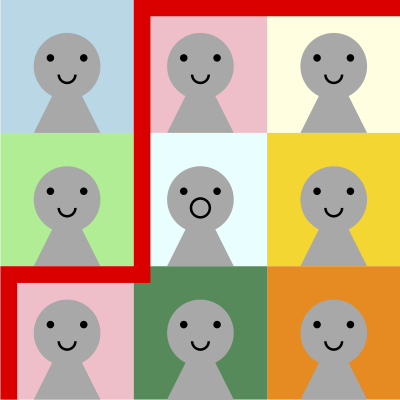
\includegraphics[scale=.40]{logoFPSAC20} \\[.5cm]
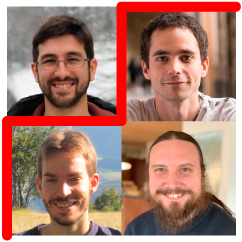
\includegraphics[scale=.69]{photos} \\[.5cm]

\includegraphics[scale=.69]{PPPP}
\end{center}
\vspace{-.6cm}
}
\end{minipage}
\hspace{1.5cm}
\begin{minipage}{20cm}
\begin{flushleft}
{\blue \fontsize{80}{45}\selectfont

On type cones \\ of g-vector fans

}

\vspace{1cm}
\HUGE{A. PADROL} \\[-.1cm]
(Sorbonne Univ.)

\vspace{.7cm}
\HUGE{Y. PALU} \\[-.1cm]
(Univ. Amiens)

\vspace{.7cm}
\HUGE{V. PILAUD} \\[-.1cm]
(CNRS \& �cole Polytechnique)

\vspace{.7cm}
\HUGE{P.-G. PLAMONDON} \\[-.1cm]
(Univ. Paris-Saclay $\to$ Univ. Versailles)

\vspace{-4.4cm}\hspace{7cm}\smash{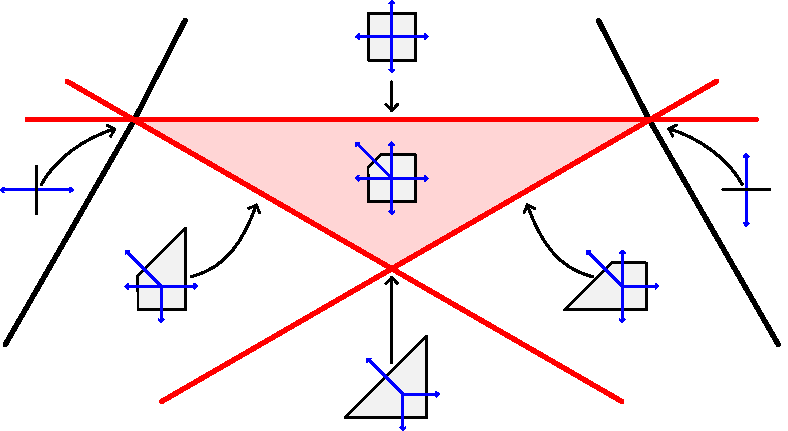
\includegraphics[scale=.9]{typeConeCoarsenings}}

\vspace{4.9cm}
\Large slides: \url{http://www.lix.polytechnique.fr/~pilaud/FPSAC20.pdf}

\Large preprint: \url{https://arxiv.org/pdf/1906.06861.pdf}

\vspace{-.6cm}

\end{flushleft}
\end{minipage}

\vspace*{-3cm}

%\begin{center}
%{\blue \fontsize{50}{45}\selectfont
%
%Type cones of g-vector fans
%
%}
%
%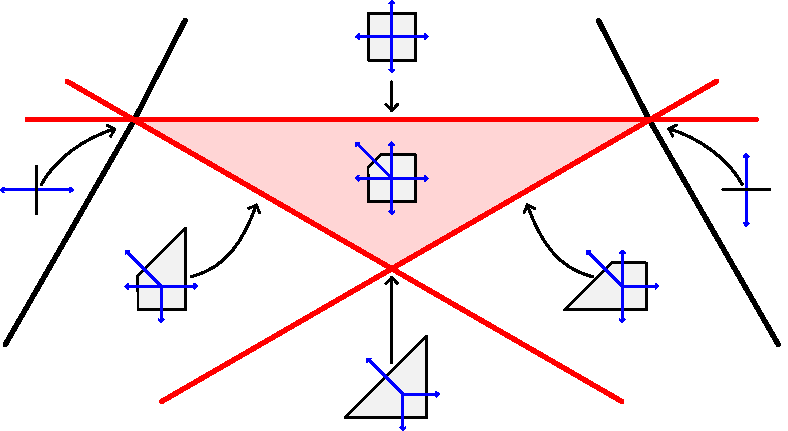
\includegraphics[scale=1.1]{typeConeCoarsenings}
%
%\begin{tabular}{c@{\qquad}c}
%\HUGE{A. PADROL} & \HUGE{Y. PALU} \\[-.1cm]
%(Sorbonne Univ.) & (Univ. Amiens) \\[1cm]
%\HUGE{V. PILAUD} & \HUGE{P.-G. PLAMONDON} \\[-.1cm]
%(CNRS \& �cole Polytechnique) & (Univ. Paris-Saclay $\to$ Univ. Versailles)
%\end{tabular}
%
%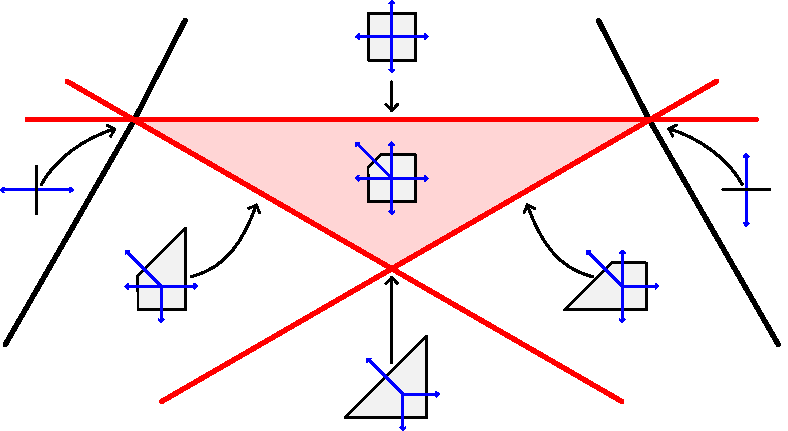
\includegraphics[scale=1.1]{typeConeCoarsenings}
%
%\end{center}


%%%%%%%%%%%%%%%%%%%%%%%%%%%%%%%%%%%%%%%%%%%%%%%%%%%%%%
%%%%%%%%%%%%%%%%%%%%%%%%%%%%%%%%%%%%%%%%%%%%%%%%%%%%%%

%%%%%%%%%%%%%%%%%%%%%%%%%%%%%%%%%%%%%%%%%%%%%%%%%%%%%%

\partie{Kinematic associahedron}

%%%%%%%%%

\begin{slide}{Associahedron}

\emph{associahedron} = polytope whose graph is the flip graph on triangulations of a polygon
%\begin{tabular}[t]{@{\;}l}
%	$n$-dimensional polytope whose graph is the flip graph \\ on triangulations of a convex $(n+3)$-gon
%\end{tabular}

\vspace{.5cm}
\centerline{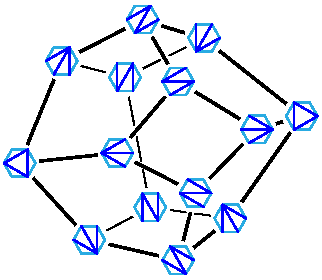
\includegraphics[scale=3.3]{associahedronSecondaryPolytope}}
\vspace*{-3.5cm}
\begin{tabular}{r@{ $\leftrightarrow$ }l}
vertices & triangulations \\
edges & flips \\
faces & dissections
\end{tabular}
\hfill
\begin{tabular}{r@{ $\leftrightarrow$ }l}
vertices & binary trees \\
edges & rotations \\
faces & Schr\"oder trees
\end{tabular}

\vspace{.8cm}
\centerline{\papier{Tamari ('51) \qquad Stasheff ('63)}}

\end{slide}

%%%

\begin{slide}{Associahedron}

\emph{associahedron} = polytope whose graph is the flip graph on triangulations of a polygon
%\begin{tabular}[t]{@{\;}l}
%	$n$-dimensional polytope whose graph is the flip graph \\ on triangulations of a convex $(n+3)$-gon
%\end{tabular}

\vspace{.5cm}
Three families of constructions (with non-equivalent normal fans):

\vspace{.5cm}
\begin{tabular}{cc|ccc|cc}
\begin{minipage}[t]{8.5cm}
\centerline{\blue SECONDARY FAN}
\vspace{.5cm}
\centerline{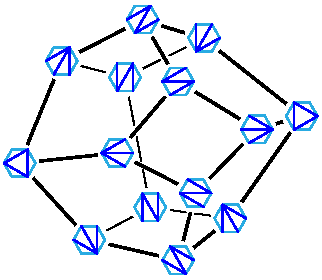
\includegraphics[scale=1.5]{associahedronSecondaryPolytope}}
\vspace{.5cm}
\papier{Gelfand--Kapranov--Zelevinsky ('94) \\ Billera--Filliman--Sturmfels ('90)

}
\end{minipage}
&&&
\begin{minipage}[t]{8.5cm}
\centerline{\blue G-VECTOR FAN}
\vspace{.5cm}
\centerline{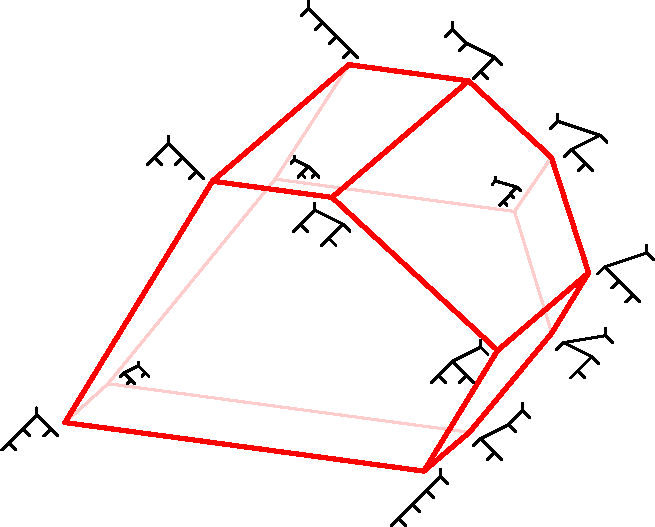
\includegraphics[scale=.78]{associahedronBinaryTrees}}
\vspace{.5cm}
\papier{Shnider--Sternberg ('93) \\ Loday ('04) \\ Hohlweg--Lange ('07) \\ Hohlweg--Lange--Thomas ('12) \\ Hohlweg--P.--Stella ('18)

}
\end{minipage}
&&&
\begin{minipage}[t]{8.5cm}
\centerline{\blue D-VECTOR FAN}
\vspace{.5cm}
\centerline{\setlength{\unitlength}{1.8pt}
\begin{picture}(90,110)(0,0) 
%\linethickness{1mm}
\thicklines 
 
 
\put(0,0){\line(1,0){60}} 
\put(0,0){\line(0,1){40}} 
\put(60,0){\line(0,1){20}} 
\put(60,0){\line(1,1){30}} 
\put(0,40){\line(1,0){40}} 
\put(0,40){\line(1,3){20}} 
\put(60,20){\line(-1,1){20}} 
\put(60,20){\line(1,3){10}} 
\put(90,30){\line(0,1){40}} 
\put(40,40){\line(1,3){10}} 
\put(70,50){\line(1,1){20}} 
\put(70,50){\line(-1,1){20}} 
\put(50,70){\line(-1,3){10}} 
\put(90,70){\line(-1,1){40}} 
\put(20,100){\line(1,0){20}} 
\put(20,100){\line(1,1){10}} 
\put(30,110){\line(1,0){20}} 
\put(40,100){\line(1,1){10}} 
 
\thinlines 
\multiput(0,0)(1.5,1.5){20}{\circle*{0.5}} 
\multiput(30,30)(2,0){30}{\circle*{0.5}} 
\multiput(30,30)(0,2){40}{\circle*{0.5}} 
 
\put(35,105){\makebox(0,0){\blue $\scriptstyle \alpha_2$}} 
\put(28,70){\makebox(0,0){\blue $\scriptstyle \alpha_1+\alpha_2$}} 
\put(63,80){\makebox(0,0){\blue $\scriptstyle \alpha_2+\alpha_3$}} 
\put(55,45){\makebox(0,0){\blue $\scriptstyle \alpha_1+\alpha_2+\alpha_3$}} 
\put(32,18){\makebox(0,0){\blue $\scriptstyle \alpha_1$}} 
\put(77,37){\makebox(0,0){\blue $\scriptstyle \alpha_3$}} 
 
 
 
%\put(0,0){\circle*{2}} 
%\put(60,0){\circle*{2}} 
%\put(60,20){\circle*{2}} 
%\put(30,30){\circle*{2}} 
%\put(90,30){\circle*{2}} 
%\put(0,40){\circle*{2}} 
%\put(40,40){\circle*{2}} 
%\put(70,50){\circle*{2}} 
%\put(50,70){\circle*{2}} 
%\put(90,70){\circle*{2}} 
%\put(20,100){\circle*{2}} 
%\put(40,100){\circle*{2}} 
%\put(30,110){\circle*{2}} 
%\put(50,110){\circle*{2}} 
\end{picture} }
\vspace{.3cm}
\hfill {\normalsize (Pictures by CFZ)} \hspace{1cm} \\[.5cm]
\papier{Chapoton--Fomin--Zelevinsky ('02) \\ Ceballos--Santos--Ziegler ('11)

}
\end{minipage}
\end{tabular}

\end{slide}

%%%

\begin{slide}{Associahedron}

\emph{associahedron} = polytope whose graph is the flip graph on triangulations of a polygon
%\begin{tabular}[t]{@{\;}l}
%	$n$-dimensional polytope whose graph is the flip graph \\ on triangulations of a convex $(n+3)$-gon
%\end{tabular}

\vspace{.5cm}
Three families of constructions (with non-equivalent normal fans):

\vspace{.5cm}
\begin{tabular}{cc|ccc|cc}
\begin{minipage}[t]{8.5cm}
\centerline{\blue SECONDARY FAN}
\vspace{.5cm}
\centerline{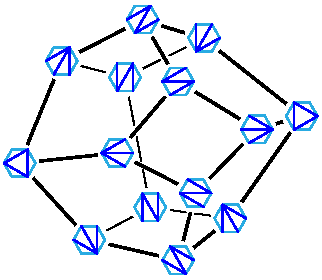
\includegraphics[scale=1.5]{associahedronSecondaryPolytope}}
\vspace{.5cm}
\papier{Gelfand--Kapranov--Zelevinsky ('94) \\ Billera--Filliman--Sturmfels ('90)

}
\end{minipage}
&&&
\begin{minipage}[t]{8.5cm}
\centerline{\blue G-VECTOR FAN}
\vspace{.5cm}
\centerline{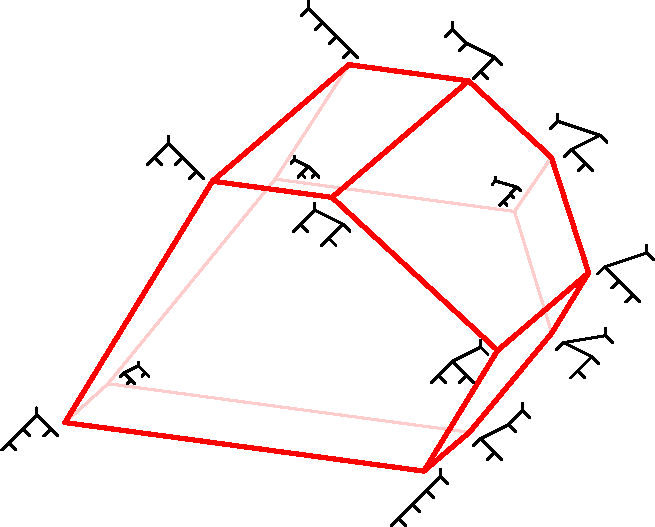
\includegraphics[scale=.78]{associahedronBinaryTrees}}
\vspace{.5cm}
\papier{Shnider--Sternberg ('93) \\ Loday ('04) \\ Hohlweg--Lange ('07) \\ Hohlweg--Lange--Thomas ('12) \\ Hohlweg--P.--Stella ('18)

}
\end{minipage}
&&&
\begin{minipage}[t]{8.5cm}
\centerline{\blue D-VECTOR FAN}
\vspace{.5cm}
\centerline{\setlength{\unitlength}{1.8pt}
\begin{picture}(90,110)(0,0) 
%\linethickness{1mm}
\thicklines 
 
 
\put(0,0){\line(1,0){60}} 
\put(0,0){\line(0,1){40}} 
\put(60,0){\line(0,1){20}} 
\put(60,0){\line(1,1){30}} 
\put(0,40){\line(1,0){40}} 
\put(0,40){\line(1,3){20}} 
\put(60,20){\line(-1,1){20}} 
\put(60,20){\line(1,3){10}} 
\put(90,30){\line(0,1){40}} 
\put(40,40){\line(1,3){10}} 
\put(70,50){\line(1,1){20}} 
\put(70,50){\line(-1,1){20}} 
\put(50,70){\line(-1,3){10}} 
\put(90,70){\line(-1,1){40}} 
\put(20,100){\line(1,0){20}} 
\put(20,100){\line(1,1){10}} 
\put(30,110){\line(1,0){20}} 
\put(40,100){\line(1,1){10}} 
 
\thinlines 
\multiput(0,0)(1.5,1.5){20}{\circle*{0.5}} 
\multiput(30,30)(2,0){30}{\circle*{0.5}} 
\multiput(30,30)(0,2){40}{\circle*{0.5}} 
 
\put(35,105){\makebox(0,0){\blue $\scriptstyle \alpha_2$}} 
\put(28,70){\makebox(0,0){\blue $\scriptstyle \alpha_1+\alpha_2$}} 
\put(63,80){\makebox(0,0){\blue $\scriptstyle \alpha_2+\alpha_3$}} 
\put(55,45){\makebox(0,0){\blue $\scriptstyle \alpha_1+\alpha_2+\alpha_3$}} 
\put(32,18){\makebox(0,0){\blue $\scriptstyle \alpha_1$}} 
\put(77,37){\makebox(0,0){\blue $\scriptstyle \alpha_3$}} 
 
 
 
%\put(0,0){\circle*{2}} 
%\put(60,0){\circle*{2}} 
%\put(60,20){\circle*{2}} 
%\put(30,30){\circle*{2}} 
%\put(90,30){\circle*{2}} 
%\put(0,40){\circle*{2}} 
%\put(40,40){\circle*{2}} 
%\put(70,50){\circle*{2}} 
%\put(50,70){\circle*{2}} 
%\put(90,70){\circle*{2}} 
%\put(20,100){\circle*{2}} 
%\put(40,100){\circle*{2}} 
%\put(30,110){\circle*{2}} 
%\put(50,110){\circle*{2}} 
\end{picture} }
\vspace{.3cm}
\hfill {\normalsize (Pictures by CFZ)} \hspace{1cm} \\[.5cm]
\papier{Chapoton--Fomin--Zelevinsky ('02) \\ Ceballos--Santos--Ziegler ('11)

}
\end{minipage}
\end{tabular}

\gboite{
	\centerline{Unidentified Construction of the Associahedron = ABHY kinematic associahedron}
	\vspace{-.1cm}
	\centerline{\papier{Arkani-Hamed--Bai--He--Yan ('18) \qquad 
Bazier-Matte--Douville--Mousavand--Thomas--Y\i{}ld\i{}r\i{}m ('18$^+$)}}
	\vspace{-.1cm}
}

\end{slide}

%%%

\begin{slide}{Kinematic associahedron}

%\emph{associahedron} = polytope whose graph is the flip graph on triangulations of a polygon

%\vspace{.3cm}
\emph{kinematic associahedron} = 
\begin{tabular}[t]{@{\;}l}
	$n$-dimensional associahedron constructed in the \\
	$n(n+3)/2$-dimensional kinematic space as a section of an \\
	$n$-dimensional affine subspace with the positive orthant
\end{tabular}

\vspace{-1.8cm} \papier{Arkani-Hamed--Bai--He--Yan ('18)}

\end{slide}

%%%

\begin{slide}{Kinematic associahedron}

%\emph{associahedron} = polytope whose graph is the flip graph on triangulations of a polygon

%\vspace{.3cm}
\emph{kinematic associahedron} = 
\begin{tabular}[t]{@{\;}l}
	$n$-dimensional associahedron constructed in the \\
	$n(n+3)/2$-dimensional kinematic space as a section of an \\
	$n$-dimensional affine subspace with the positive orthant
\end{tabular}

\vspace{-1.8cm} \papier{Arkani-Hamed--Bai--He--Yan ('18)}

\vspace{1.3cm}
fix parameters $\b{\ell}_A, \dots, \b{\ell}_F > 0$ \\
$\b{z} \ge 0$ indexed by internal diagonals of $(n+3)$-gon

\vspace{-2.5cm}\hspace{-.6cm}
\begin{tikzpicture}
	\matrix (m) [matrix of math nodes, row sep=.7cm, column sep=.3cm, nodes={anchor=center, align=center, inner sep=0pt}]{
		&& \;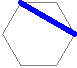
\includegraphics[scale=1.3]{diagonalB3} & \node (c) {\red \circled{C}}; & \;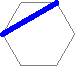
\includegraphics[scale=1.3]{diagonalB7} && \\
		& \;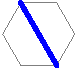
\includegraphics[scale=1.3]{diagonalB2} & \node (b) {\red \circled{B}}; & \;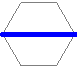
\includegraphics[scale=1.3]{diagonalB5} & \node (e) {\red \circled{E}}; & \;
\includegraphics[scale=1.3]{diagonalB8} & \\
		\;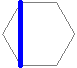
\includegraphics[scale=1.3]{diagonalB1} & \node (a) {\red \circled{A}}; & \;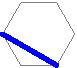
\includegraphics[scale=1.3]{diagonalB4} & \node (d) {\red \circled{D}}; & \;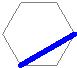
\includegraphics[scale=1.3]{diagonalB6} & \node (f) {\red \circled{F}}; & \;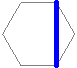
\includegraphics[scale=1.3]{diagonalB9} \\};
	\draw[->] (m-3-1) -- (m-2-2);
	\draw[->] (m-2-2) -- (m-1-3);
	\draw[->] (m-2-2) -- (m-3-3);
	\draw[->] (m-1-3) -- (m-2-4);
	\draw[->] (m-3-3) -- (m-2-4);
	\draw[->] (m-2-4) -- (m-1-5);
	\draw[->] (m-2-4) -- (m-3-5);
	\draw[->] (m-1-5) -- (m-2-6);
	\draw[->] (m-3-5) -- (m-2-6);
	\draw[->] (m-2-6) -- (m-3-7);
	\draw[red] (a) -- (m-3-1);
	\draw[red] (a) -- (m-3-3);
	\draw[red] (a) -- (m-2-2);
	\draw[red] (b) -- (m-2-2);
	\draw[red] (b) -- (m-2-4);
	\draw[red] (b) -- (m-1-3);
	\draw[red] (b) -- (m-3-3);
	\draw[red] (c) -- (m-1-3);
	\draw[red] (c) -- (m-1-5);
	\draw[red] (c) -- (m-2-4);
	\draw[red] (d) -- (m-3-3);
	\draw[red] (d) -- (m-3-5);
	\draw[red] (d) -- (m-2-4);
	\draw[red] (e) -- (m-2-4);
	\draw[red] (e) -- (m-2-6);
	\draw[red] (e) -- (m-1-5);
	\draw[red] (e) -- (m-3-5);
	\draw[red] (f) -- (m-3-5);
	\draw[red] (f) -- (m-3-7);
	\draw[red] (f) -- (m-2-6);
\end{tikzpicture}
%
\hspace{-.5cm}
\raisebox{4.5cm}{
\begin{minipage}{6cm}
\begin{align*}
%	\b{z} & \ge \b{0} \\
	\b{z}_{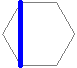
\includegraphics[scale=.7]{diagonalB1}} + \b{z}_{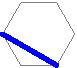
\includegraphics[scale=.7]{diagonalB4}} - \b{z}_{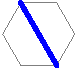
\includegraphics[scale=.7]{diagonalB2}} & = \b{\ell}_A \\
	\b{z}_{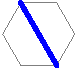
\includegraphics[scale=.7]{diagonalB2}} + \b{z}_{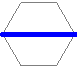
\includegraphics[scale=.7]{diagonalB5}} - \b{z}_{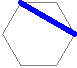
\includegraphics[scale=.7]{diagonalB3}} - \b{z}_{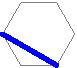
\includegraphics[scale=.7]{diagonalB4}} & = \b{\ell}_B \\
	\b{z}_{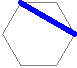
\includegraphics[scale=.7]{diagonalB3}} + \b{z}_{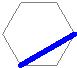
\includegraphics[scale=.7]{diagonalB6}} - \b{z}_{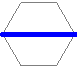
\includegraphics[scale=.7]{diagonalB5}} & = \b{\ell}_C \\
	\b{z}_{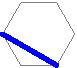
\includegraphics[scale=.7]{diagonalB4}} + \b{z}_{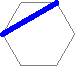
\includegraphics[scale=.7]{diagonalB7}} - \b{z}_{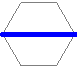
\includegraphics[scale=.7]{diagonalB5}} & = \b{\ell}_D \\
	\b{z}_{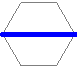
\includegraphics[scale=.7]{diagonalB5}} + \b{z}_{
\includegraphics[scale=.7]{diagonalB8}} - \b{z}_{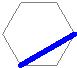
\includegraphics[scale=.7]{diagonalB6}} - \b{z}_{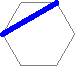
\includegraphics[scale=.7]{diagonalB7}} & = \b{\ell}_E \\
	\b{z}_{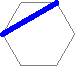
\includegraphics[scale=.7]{diagonalB7}} + \b{z}_{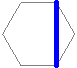
\includegraphics[scale=.7]{diagonalB9}} - \b{z}_{
\includegraphics[scale=.7]{diagonalB8}} & = \b{\ell}_F
\end{align*}
\end{minipage}
}

\end{slide}

%%%

\begin{slide}{Kinematic associahedron}

%\emph{associahedron} = polytope whose graph is the flip graph on triangulations of a polygon

%\vspace{.3cm}
\emph{kinematic associahedron} = 
\begin{tabular}[t]{@{\;}l}
	$n$-dimensional associahedron constructed in the \\
	$n(n+3)/2$-dimensional kinematic space as a section of an \\
	$n$-dimensional affine subspace with the positive orthant
\end{tabular}

\vspace{-1.8cm} \papier{Arkani-Hamed--Bai--He--Yan ('18)}

\vspace{1.3cm}
fix parameters $\b{\ell}_A, \dots, \b{\ell}_F > 0$ \\
$\b{z} \ge 0$ indexed by internal diagonals of $(n+3)$-gon

\vspace{-2.5cm}\hspace{-.6cm}
\begin{tikzpicture}
	\matrix (m) [matrix of math nodes, row sep=.7cm, column sep=.3cm, nodes={anchor=center, align=center, inner sep=0pt}]{
		&& \;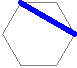
\includegraphics[scale=1.3]{diagonalB3} & \node (c) {\red \circled{C}}; & \;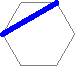
\includegraphics[scale=1.3]{diagonalB7} && \\
		& \;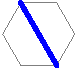
\includegraphics[scale=1.3]{diagonalB2} & \node (b) {\red \circled{B}}; & \;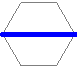
\includegraphics[scale=1.3]{diagonalB5} & \node (e) {\red \circled{E}}; & \;
\includegraphics[scale=1.3]{diagonalB8} & \\
		\;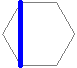
\includegraphics[scale=1.3]{diagonalB1} & \node (a) {\red \circled{A}}; & \;\includegraphics[scale=1.3]{diagonalB4} & \node (d) {\red \circled{D}}; & \;\includegraphics[scale=1.3]{diagonalB6} & \node (f) {\red \circled{F}}; & \;\includegraphics[scale=1.3]{diagonalB9} \\};
	\draw[->] (m-3-1) -- (m-2-2);
	\draw[->] (m-2-2) -- (m-1-3);
	\draw[->] (m-2-2) -- (m-3-3);
	\draw[->] (m-1-3) -- (m-2-4);
	\draw[->] (m-3-3) -- (m-2-4);
	\draw[->] (m-2-4) -- (m-1-5);
	\draw[->] (m-2-4) -- (m-3-5);
	\draw[->] (m-1-5) -- (m-2-6);
	\draw[->] (m-3-5) -- (m-2-6);
	\draw[->] (m-2-6) -- (m-3-7);
	\draw[red] (a) -- (m-3-1);
	\draw[red] (a) -- (m-3-3);
	\draw[red] (a) -- (m-2-2);
	\draw[red] (b) -- (m-2-2);
	\draw[red] (b) -- (m-2-4);
	\draw[red] (b) -- (m-1-3);
	\draw[red] (b) -- (m-3-3);
	\draw[red] (c) -- (m-1-3);
	\draw[red] (c) -- (m-1-5);
	\draw[red] (c) -- (m-2-4);
	\draw[red] (d) -- (m-3-3);
	\draw[red] (d) -- (m-3-5);
	\draw[red] (d) -- (m-2-4);
	\draw[red] (e) -- (m-2-4);
	\draw[red] (e) -- (m-2-6);
	\draw[red] (e) -- (m-1-5);
	\draw[red] (e) -- (m-3-5);
	\draw[red] (f) -- (m-3-5);
	\draw[red] (f) -- (m-3-7);
	\draw[red] (f) -- (m-2-6);
\end{tikzpicture}
%
\hspace{-.5cm}
\raisebox{4.5cm}{
\begin{minipage}{6cm}
\begin{align*}
%	\b{z} & \ge \b{0} \\
	\b{z}_{\includegraphics[scale=.7]{diagonalB1}} + \b{z}_{\includegraphics[scale=.7]{diagonalB4}} - \b{z}_{\includegraphics[scale=.7]{diagonalB2}} & = \b{\ell}_A \\
	\b{z}_{\includegraphics[scale=.7]{diagonalB2}} + \b{z}_{\includegraphics[scale=.7]{diagonalB5}} - \b{z}_{\includegraphics[scale=.7]{diagonalB3}} - \b{z}_{\includegraphics[scale=.7]{diagonalB4}} & = \b{\ell}_B \\
	\b{z}_{\includegraphics[scale=.7]{diagonalB3}} + \b{z}_{\includegraphics[scale=.7]{diagonalB6}} - \b{z}_{\includegraphics[scale=.7]{diagonalB5}} & = \b{\ell}_C \\
	\b{z}_{\includegraphics[scale=.7]{diagonalB4}} + \b{z}_{\includegraphics[scale=.7]{diagonalB7}} - \b{z}_{\includegraphics[scale=.7]{diagonalB5}} & = \b{\ell}_D \\
	\b{z}_{\includegraphics[scale=.7]{diagonalB5}} + \b{z}_{\includegraphics[scale=.7]{diagonalB8}} - \b{z}_{\includegraphics[scale=.7]{diagonalB6}} - \b{z}_{\includegraphics[scale=.7]{diagonalB7}} & = \b{\ell}_E \\
	\b{z}_{\includegraphics[scale=.7]{diagonalB7}} + \b{z}_{\includegraphics[scale=.7]{diagonalB9}} - \b{z}_{\includegraphics[scale=.7]{diagonalB8}} & = \b{\ell}_F
\end{align*}
\end{minipage}
}

\vspace{-.1cm}
\gboite{
	Let $X(n) = \set{(a,b)}{0 \le a < b \le n+2}$ and $Y(n) = \set{(a,b)}{1 \le a < b \le n+1}$. \\
	For any~$\b{\ell} \in \R_{>0}^{Y(n)}$, the polytope
	\[
	\set{\b{z} \in \R^{X(n)}}{\begin{array}{@{}l} \b{z} \ge 0, \quad \b{z}_{(0,n+2)} = 0 \quad\text{and}\quad \b{z}_{(a,a+1)} = 0 \text{ for all } 0 \le a \le n+1 \\ \b{z}_{(a-1,b)} + \b{z}_{(a,b+1)} - \b{z}_{(a,b)} - \b{z}_{(a-1,b+1)} = \b{\ell}_{(a,b)} \text{ for all } (a,b) \in Y(n) \end{array}}
	\]
	is an associahedron. \hfill \papier{Arkani-Hamed--Bai--He--Yan ('18)}
	\vspace{-.1cm}
}

\end{slide}

%%%%%%%%%%%%%%%%%%%%%%%%%%%%%%%%%%%%%%%%%%%%%%%%%%%%%%

\partie{Type cones}

%%%%%%%%%

\begin{slide}{Choosing right-hand-sides}

$\c{F}$ = complete simplicial fan in~$\R^n$ with~$N$ rays \\
$\b{G}$ = $(N \times n)$-matrix whose rows are representatives of the rays of~$\c{F}$ \\
for a height vector~$\b{h} \in \R_{>0}^N$, consider the polytope~$\poly{P}_{\b{h}} = \set{\b{x} \in \R^n}{\b{G}\b{x} \le \b{h}}$

\vspace{1cm}
\centerline{
	\begin{tabular}{c@{\quad}c@{\quad}c@{\quad}c}
		\includegraphics[scale=1.5]{typeConeFan} & \includegraphics[scale=1.5]{typeConePolytope1a} & \includegraphics[scale=1.5]{typeConePolytope2a} & \includegraphics[scale=1.5]{typeConePolytope3a} \\
		& A & B & C
	\end{tabular}
}
\centerline{}

\end{slide}

%%%

\begin{slide}{Choosing right-hand-sides}

$\c{F}$ = complete simplicial fan in~$\R^n$ with~$N$ rays \\
$\b{G}$ = $(N \times n)$-matrix whose rows are representatives of the rays of~$\c{F}$ \\
for a height vector~$\b{h} \in \R_{>0}^N$, consider the polytope~$\poly{P}_{\b{h}} = \set{\b{x} \in \R^n}{\b{G}\b{x} \le \b{h}}$

\vspace{1cm}
\centerline{
	\begin{tabular}{c@{\quad}c@{\quad}c@{\quad}c}
		\includegraphics[scale=1.5]{typeConeFan} & \includegraphics[scale=1.5]{typeConePolytope1b} & \includegraphics[scale=1.5]{typeConePolytope2b} & \includegraphics[scale=1.5]{typeConePolytope3b} \\
		& A & B & C
	\end{tabular}
}

\end{slide}

%%%

\begin{slide}{Choosing right-hand-sides}

$\c{F}$ = complete simplicial fan in~$\R^n$ with~$N$ rays \\
$\b{G}$ = $(N \times n)$-matrix whose rows are representatives of the rays of~$\c{F}$ \\
for a height vector~$\b{h} \in \R_{>0}^N$, consider the polytope~$\poly{P}_{\b{h}} = \set{\b{x} \in \R^n}{\b{G}\b{x} \le \b{h}}$

\vspace{1cm}
\centerline{
	\begin{tabular}{c@{\quad}c@{\quad}c@{\quad}c}
		\includegraphics[scale=1.5]{typeConeFan} & \includegraphics[scale=1.5]{typeConePolytope1b} & \includegraphics[scale=1.5]{typeConePolytope2b} & \includegraphics[scale=1.5]{typeConePolytope3b} \\
		& A & B & C
	\end{tabular}
}

\vspace{.3cm}
When is~$\c{F}$ the normal fan of~$\poly{P}_{\b{h}}$?

\end{slide}

%%%

\begin{slide}{Choosing right-hand-sides}

$\c{F}$ = complete simplicial fan in~$\R^n$ with~$N$ rays \\
$\b{G}$ = $(N \times n)$-matrix whose rows are representatives of the rays of~$\c{F}$ \\
for a height vector~$\b{h} \in \R_{>0}^N$, consider the polytope~$\poly{P}_{\b{h}} = \set{\b{x} \in \R^n}{\b{G}\b{x} \le \b{h}}$

\vspace{1cm}
\centerline{
	\begin{tabular}{c@{\quad}c@{\quad}c@{\quad}c}
		\includegraphics[scale=1.5]{typeConeFan} & \includegraphics[scale=1.5]{typeConePolytope1b} & \includegraphics[scale=1.5]{typeConePolytope2b} & \includegraphics[scale=1.5]{typeConePolytope3b} \\
		& A & B & C
	\end{tabular}
}

\vspace{.3cm}
When is~$\c{F}$ the normal fan of~$\poly{P}_{\b{h}}$?

\vspace{.5cm}
$\poly{P}$ polytope, $\poly{F}$ face of~$\poly{P}$ \\[.2cm]
\emph{normal cone} of~$\poly{F}$ = 
\begin{tabular}[t]{@{\;}l}
	positive span of the outer normal \\
	vectors of the facets containing~$\poly{F}$
\end{tabular} \\[.5cm]
\emph{normal fan} of~$\poly{P}$ = $\{$ normal cone of~$\poly{F}$ $|$ $\poly{F}$ face of~$\poly{P}$ $\}$

\vspace{-6cm}\hspace{17cm}
\includegraphics[scale=.7]{normalFanCube}

\end{slide}

%%%

\begin{slide}{Wall-crossing inequalities}

$\c{F}$ = complete simplicial fan in~$\R^n$ with~$N$ rays \\
$\b{G}$ = $(N \times n)$-matrix whose rows are representatives of the rays of~$\c{F}$ \\
for a height vector~$\b{h} \in \R_{>0}^N$, consider the polytope~$\poly{P}_{\b{h}} = \set{\b{x} \in \R^n}{\b{G}\b{x} \le \b{h}}$

\centerline{\includegraphics[scale=1.7]{wallCrossingInequality1}}

\end{slide}

%%%

\begin{slide}{Wall-crossing inequalities}

$\c{F}$ = complete simplicial fan in~$\R^n$ with~$N$ rays \\
$\b{G}$ = $(N \times n)$-matrix whose rows are representatives of the rays of~$\c{F}$ \\
for a height vector~$\b{h} \in \R_{>0}^N$, consider the polytope~$\poly{P}_{\b{h}} = \set{\b{x} \in \R^n}{\b{G}\b{x} \le \b{h}}$

\centerline{\includegraphics[scale=1.7]{wallCrossingInequality2}}

\end{slide}

%%%

\begin{slide}{Wall-crossing inequalities}

$\c{F}$ = complete simplicial fan in~$\R^n$ with~$N$ rays \\
$\b{G}$ = $(N \times n)$-matrix whose rows are representatives of the rays of~$\c{F}$ \\
for a height vector~$\b{h} \in \R_{>0}^N$, consider the polytope~$\poly{P}_{\b{h}} = \set{\b{x} \in \R^n}{\b{G}\b{x} \le \b{h}}$

\centerline{\includegraphics[scale=1.7]{wallCrossingInequality2}}

\gboite{
\emph{wall-crossing inequality} for a wall~$\b{R}$ = \qquad $\displaystyle \smashoperator{\sum_{\b{s} \in \b{R} \, \cup \{\b{r}, \b{r}'\}}} \alpha_{\b{R},\b{s}} \, \b{h}_{\b{s}} > 0$ \qquad where \\[-.2cm]
\begin{compactitem}
\item $\b{r}, \b{r'}$ = rays such that~$\b{R} \cup \{\b{r}\}$ and~$\b{R} \cup \{\b{r}'\}$ are chambers of~$\c{F}$
\item $\alpha_{\b{R},\b{s}}$ = coeff. of unique linear dependence $\displaystyle \smashoperator{\sum_{\b{s} \in \b{R} \, \cup \{\b{r}, \b{r}'\}}} \alpha_{\b{R},\b{s}} \, \b{s} = 0$ with $\alpha_{\b{R},\b{r}} + \alpha_{\b{R},\b{r}'} = 2$
\end{compactitem}
\vspace{-.3cm}
}

\end{slide}

%%%

\begin{slide}{Wall-crossing inequalities}

$\c{F}$ = complete simplicial fan in~$\R^n$ with~$N$ rays \\
$\b{G}$ = $(N \times n)$-matrix whose rows are representatives of the rays of~$\c{F}$ \\
for a height vector~$\b{h} \in \R_{>0}^N$, consider the polytope~$\poly{P}_{\b{h}} = \set{\b{x} \in \R^n}{\b{G}\b{x} \le \b{h}}$

\centerline{\includegraphics[scale=1.7]{wallCrossingInequality2}}

\gboite{
\emph{wall-crossing inequality} for a wall~$\b{R}$ = \qquad $\displaystyle \smashoperator{\sum_{\b{s} \in \b{R} \, \cup \{\b{r}, \b{r}'\}}} \alpha_{\b{R},\b{s}} \, \b{h}_{\b{s}} > 0$ \qquad where \\[-.2cm]
\begin{compactitem}
\item $\b{r}, \b{r'}$ = rays such that~$\b{R} \cup \{\b{r}\}$ and~$\b{R} \cup \{\b{r}'\}$ are chambers of~$\c{F}$
\item $\alpha_{\b{R},\b{s}}$ = coeff. of unique linear dependence $\displaystyle \smashoperator{\sum_{\b{s} \in \b{R} \, \cup \{\b{r}, \b{r}'\}}} \alpha_{\b{R},\b{s}} \, \b{s} = 0$ with $\alpha_{\b{R},\b{r}} + \alpha_{\b{R},\b{r}'} = 2$
\end{compactitem}
\vspace{-.3cm}
}

\gboite{
\centerline{$\c{F}$ is the normal fan of~$\poly{P}_{\b{h}}$ $\iff$ $\b{h}$ satisfies all wall-crossing inequalities of~$\c{F}$}
}

\end{slide}

%%%

\begin{slide}{Wall-crossing inequalities}

$\c{F}$ = complete simplicial fan in~$\R^n$ with~$N$ rays \\
$\b{G}$ = $(N \times n)$-matrix whose rows are representatives of the rays of~$\c{F}$ \\
for a height vector~$\b{h} \in \R_{>0}^N$, consider the polytope~$\poly{P}_{\b{h}} = \set{\b{x} \in \R^n}{\b{G}\b{x} \le \b{h}}$

\vspace{1cm}
\centerline{
	\begin{tabular}{c@{\quad}c@{\quad}c@{\quad}c}
		\includegraphics[scale=1.5]{typeConeFan} & \includegraphics[scale=1.5]{typeConePolytope1b} & \includegraphics[scale=1.5]{typeConePolytope2b} & \includegraphics[scale=1.5]{typeConePolytope3b} \\
		& A & B & C
	\end{tabular}
}

\vspace{-.1cm}
wall-crossing inequalities: \\[-.2cm]
\begin{minipage}{14cm}
\begin{align*}
\text{wall } 1: & \quad h_2 + h_5 > 0
\\
\text{wall } 2: & \quad h_1 + h_3 > h_2
\\
\text{wall } 3: & \quad h_2 + h_4 > h_3
\\
\text{wall } 4: & \quad h_3 + h_5 > h_4
\\
\text{wall } 5: & \quad h_1 + h_4 > 0
\end{align*}
\end{minipage}
\raisebox{-3cm}{\includegraphics[scale=.8]{typeConeABC}}

\end{slide}

%%%%%%%%%

\begin{slide}{Type cone}

$\c{F}$ = complete simplicial fan in~$\R^n$ with~$N$ rays \\
$\b{G}$ = $(N \times n)$-matrix whose rows are representatives of the rays of~$\c{F}$ \\
for a height vector~$\b{h} \in \R_{>0}^N$, consider the polytope~$\poly{P}_{\b{h}} = \set{\b{x} \in \R^n}{\b{G}\b{x} \le \b{h}}$

\gboite{
\emph{type cone}~$\typeCone(\c{F})$ 
\begin{tabular}[t]{@{\;}l}
	= realization space of~$\c{F}$ \\
	= $\set{\b{h} \in \R^N}{\c{F} \text{ is the normal fan of } \poly{P}_{\b{h}}}$ \\
	= $\set{\b{h} \in \R^N}{\b{h} \text{ satisfies all wall-crossing inequalities of } \c{F}}$
\end{tabular}
\hspace{-10cm}\hfill \papier{McMullen ('73)} 
}

\vspace{.2cm}
\centerline{\includegraphics[scale=1.5]{typeConeFan} \qquad \raisebox{.5cm}{\includegraphics[scale=.8]{typeCone}}}

%some properties of $\typeCone(\c{F})$:
%\begin{compactitem}
%\item $\typeCone(\c{F})$ is an open cone \hspace{3.6cm} (dilations preserve normal fans)
%\item $\typeCone(\c{F})$ has lineality space~$\b{G} \, \R^n$ \hspace{1cm} (translations preserve normal fans)
%\item dimension of $\typeCone(\c{F}) / \b{G} \, \R^n$ = $N-n$
%%\item Minkowski sums $\longleftrightarrow$ convex combinations
%\end{compactitem}

\end{slide}

%%%

\begin{slide}{Type cone}

$\c{F}$ = complete simplicial fan in~$\R^n$ with~$N$ rays \\
$\b{G}$ = $(N \times n)$-matrix whose rows are representatives of the rays of~$\c{F}$ \\
for a height vector~$\b{h} \in \R_{>0}^N$, consider the polytope~$\poly{P}_{\b{h}} = \set{\b{x} \in \R^n}{\b{G}\b{x} \le \b{h}}$

\gboite{
\emph{type cone}~$\typeCone(\c{F})$
\begin{tabular}[t]{@{\;}l}
	= realization space of~$\c{F}$ \\
	= $\set{\b{h} \in \R^N}{\c{F} \text{ is the normal fan of } \poly{P}_{\b{h}}}$ \\
	= $\set{\b{h} \in \R^N}{\b{h} \text{ satisfies all wall-crossing inequalities of } \c{F}}$
\end{tabular}
\hspace{-10cm}\hfill \papier{McMullen ('73)} 
}

\vspace{.2cm}
\centerline{\includegraphics[scale=1.5]{typeConeFan} \qquad \raisebox{.5cm}{\includegraphics[scale=.8]{typeCone}}}

some properties of $\typeCone(\c{F})$:
\begin{compactitem}
\item $\typeCone(\c{F})$ is an open cone \hspace{3.6cm} (dilations preserve normal fans)
\item $\typeCone(\c{F})$ has lineality space~$\b{G} \, \R^n$ \hspace{1cm} (translations preserve normal fans)
\item dimension of $\typeCone(\c{F}) / \b{G} \, \R^n$ = $N-n$
%\item Minkowski sums $\longleftrightarrow$ convex combinations
\end{compactitem}

\end{slide}

%%%

\begin{slide}{Type cone}

$\c{F}$ = complete simplicial fan in~$\R^n$ with~$N$ rays \\
$\b{G}$ = $(N \times n)$-matrix whose rows are representatives of the rays of~$\c{F}$ \\
for a height vector~$\b{h} \in \R_{>0}^N$, consider the polytope~$\poly{P}_{\b{h}} = \set{\b{x} \in \R^n}{\b{G}\b{x} \le \b{h}}$

\gboite{
\emph{type cone}~$\typeCone(\c{F})$
\begin{tabular}[t]{@{\;}l}
	= realization space of~$\c{F}$ \\
	= $\set{\b{h} \in \R^N}{\c{F} \text{ is the normal fan of } \poly{P}_{\b{h}}}$ \\
	= $\set{\b{h} \in \R^N}{\b{h} \text{ satisfies all wall-crossing inequalities of } \c{F}}$
\end{tabular}
\hspace{-10cm}\hfill \papier{McMullen ('73)} 
}

\vspace{.2cm}
\centerline{\includegraphics[scale=1.5]{typeConeFan} \qquad \raisebox{.5cm}{\includegraphics[scale=.8]{typeConeCoarsenings}}}

some properties of $\typeCone(\c{F})$:
\begin{compactitem}
%\item $\typeCone(\c{F})$ is an open cone \hspace{3.6cm} (dilations preserve normal fans)
%\item $\typeCone(\c{F})$ has lineality space~$\b{G} \, \R^n$ \hspace{1cm} (translations preserve normal fans)
%\item dimension of $\typeCone(\c{F}) / \b{G} \, \R^n$ = $N-n$
\item boundary of~$\typeCone(\c{F})$ = polytopes whose normal fan coarsens~$\c{F}$ = deformation cone
\item Minkowski sums $\longleftrightarrow$ positive linear combinations
\end{compactitem}

\end{slide}

%%%%%%%%%

\begin{slide}{Exm: submodular functions}

\centerline{
	\begin{tabular}{l@{\qquad}l}
		\includegraphics[scale=1.3]{braidFan}
		&
		\includegraphics[scale=1.3]{permutahedron}
		\\[-.3cm]
		\emph{braid fan} = 
		&
		\emph{permutahedron} = 
		\\
		$\quad \poly{C}(\sigma) = \set{\b{x} \in \R^n}{x_{\sigma(1)} \le \dots \le x_{\sigma(n)}}$
		&
		$\quad \conv \set{[\sigma^{-1}(i)]_{i \in [n]}}{\sigma \in \fS_n}$
	\end{tabular}
}

\end{slide}

%%%

\begin{slide}{Exm: submodular functions}

\centerline{
	\begin{tabular}{l@{\qquad}l}
		\includegraphics[scale=1.3]{braidFan}
		&
		\includegraphics[scale=1.3]{permutahedron}
		\\[-.3cm]
		\emph{braid fan} = 
		&
		\emph{permutahedron} = 
		\\
		$\quad \poly{C}(\sigma) = \set{\b{x} \in \R^n}{x_{\sigma(1)} \le \dots \le x_{\sigma(n)}}$
		&
		$\quad \conv \set{[\sigma^{-1}(i)]_{i \in [n]}}{\sigma \in \fS_n}$
	\end{tabular}
}

\vspace{.1cm}
\gboite{
	\centerline{closed type cone of braid fan = $\{$deformed permutahedra$\}$ = $\{$submodular functions$\}$}
	\vspace{-.1cm}
}

\end{slide}

%%%

\begin{slide}{Exm: submodular functions}

\centerline{
	\begin{tabular}{l@{\qquad}l}
		\includegraphics[scale=1.3]{braidFan}
		&
		\includegraphics[scale=1.3]{permutahedron}
		\\[-.3cm]
		\emph{braid fan} = 
		&
		\emph{permutahedron} = 
		\\
		$\quad \poly{C}(\sigma) = \set{\b{x} \in \R^n}{x_{\sigma(1)} \le \dots \le x_{\sigma(n)}}$
		&
		$\quad \conv \set{[\sigma^{-1}(i)]_{i \in [n]}}{\sigma \in \fS_n}$
	\end{tabular}
}

\vspace{.1cm}
\gboite{
	\emph{deformed permutahedron} = polytope whose normal fan coarsens the braid fan
	\[
	\deformedPermutahedron(\b{z}) = \bigset{\b{x} \in \R_{\phantom{\ge0}}^n}{ \dotprod{\one}{\b{x}} = \b{z}_{[n]} \text{ and } \dotprod{\one_R}{\b{x}} \ge \b{z}_R \text{ for all } R \! \subseteq \! [n]}
	\]
	for some vector~$\b{z} \in \R^{2^{[n]}}$ such that~$\b{z}_R + \b{z}_S \le \b{z}_{R \cup S} + \b{z}_{R \cap S}$ and~$\b{z}_\varnothing = 0$ \\
	\phantom{where~$\c{J} = \set{J \subset [n]}{|J| \ge 2}$} \hfill \papier{Postnikov ('09) \quad Postnikov--Reiner--Williams ('08)}
	\vspace{-.1cm}	
}

\end{slide}

%%%%%%%%%

\begin{slide}{Simplicial type cone}

$\c{F}$ = complete simplicial fan in~$\R^n$ with~$N$ rays \\
$\b{G}$ = $(N \times n)$-matrix whose rows are representatives of the rays of~$\c{F}$ \\
$\b{K}$ = $(N-n) \times N$-matrix that spans the left kernel of~$\b{G}$ (ie. $\b{K}\b{G} = \b{0}$)

\end{slide}

%%%

\begin{slide}{Simplicial type cone}

$\c{F}$ = complete simplicial fan in~$\R^n$ with~$N$ rays \\
$\b{G}$ = $(N \times n)$-matrix whose rows are representatives of the rays of~$\c{F}$ \\
$\b{K}$ = $(N-n) \times N$-matrix that spans the left kernel of~$\b{G}$ (ie. $\b{K}\b{G} = \b{0}$)

\vspace{.8cm}
Classical affine transformation on polytopes:
\[
\begin{array}{ccc}
\poly{P}_{\b{h}} = \set{\b{x} \in \R^n}{\b{G}\b{x} \le \b{h}} & \longrightarrow & \poly{Q}_{\b{h}} = \set{\b{z} \in \R^N}{\b{K}\b{z} = \b{K}\b{h} \text{ and } \b{z} \ge 0} \\
\b{x} & \longmapsto & \b{z} = \b{h} - \b{G} \b{x}
\end{array}
\]

\end{slide}

%%%

\begin{slide}{Simplicial type cone}

$\c{F}$ = complete simplicial fan in~$\R^n$ with~$N$ rays \\
$\b{G}$ = $(N \times n)$-matrix whose rows are representatives of the rays of~$\c{F}$ \\
$\b{K}$ = $(N-n) \times N$-matrix that spans the left kernel of~$\b{G}$ (ie. $\b{K}\b{G} = \b{0}$)

\vspace{.8cm}
Classical affine transformation on polytopes:
\[
\begin{array}{ccc}
\poly{P}_{\b{h}} = \set{\b{x} \in \R^n}{\b{G}\b{x} \le \b{h}} & \longrightarrow & \poly{Q}_{\b{h}} = \set{\b{z} \in \R^N}{\b{K}\b{z} = \b{K}\b{h} \text{ and } \b{z} \ge 0} \\
\b{x} & \longmapsto & \b{z} = \b{h} - \b{G} \b{x}
\end{array}
\]

\vspace{-.3cm}
\gboite{
All polytopal realizations of~$\c{F}$ are affinely equivalent to
\vspace{-.2cm}
\[
\poly{Q}_{\b{h}} = \set{\b{z} \in \R^N}{\b{K}\b{z} = \b{K}\b{h} \text{ and } \b{z} \ge 0}
\]

\vspace{-.2cm}
for any~$\b{h}$ in the type cone~$\typeCone(\c{F})$.
\vspace{-.2cm}
}


\end{slide}

%%%

\begin{slide}{Simplicial type cone}

$\c{F}$ = complete simplicial fan in~$\R^n$ with~$N$ rays \\
$\b{G}$ = $(N \times n)$-matrix whose rows are representatives of the rays of~$\c{F}$ \\
$\b{K}$ = $(N-n) \times N$-matrix that spans the left kernel of~$\b{G}$ (ie. $\b{K}\b{G} = \b{0}$)

\vspace{.8cm}
Classical affine transformation on polytopes:
\[
\begin{array}{ccc}
\poly{P}_{\b{h}} = \set{\b{x} \in \R^n}{\b{G}\b{x} \le \b{h}} & \longrightarrow & \poly{Q}_{\b{h}} = \set{\b{z} \in \R^N}{\b{K}\b{z} = \b{K}\b{h} \text{ and } \b{z} \ge 0} \\
\b{x} & \longmapsto & \b{z} = \b{h} - \b{G} \b{x}
\end{array}
\]

\vspace{-.3cm}
\gboite{
All polytopal realizations of~$\c{F}$ are affinely equivalent to
\vspace{-.2cm}
\[
\poly{Q}_{\b{h}} = \set{\b{z} \in \R^N}{\b{K}\b{z} = \b{K}\b{h} \text{ and } \b{z} \ge 0}
\]

\vspace{-.2cm}
for any~$\b{h}$ in the type cone~$\typeCone(\c{F})$.
\vspace{-.2cm}
}

\gboite{
Assume that the type cone~$\typeCone(\c{F})$ is simplicial. \\
$\b{K}$ = $(N-n) \times N$-matrix whose rows are inner normal vectors of the facets of~$\typeCone(\Fan)$. \\
All polytopal realizations of~$\c{F}$ are affinely equivalent to
\vspace{-.2cm}
\[
\poly{R}_{\b{\ell}} = \set{\b{z} \in \R^N}{\b{K} \b{z} = \b{\ell} \text{ and } \b{z} \ge 0}
\]

\vspace{-.2cm}
for any positive vector~$\b{\ell} \in \R_{>0}^{N-n}$.
\hfill\papier{Padrol--Palu--P.--Plamondon ('19$^+$)}
\vspace{-.2cm}

}

\end{slide}

%%%

\begin{slide}{Simplicial type cone}

\gboite{
Assume that the type cone~$\typeCone(\c{F})$ is simplicial. \\
$\b{K}$ = $(N-n) \times N$-matrix whose rows are inner normal vectors of the facets of~$\typeCone(\Fan)$. \\
All polytopal realizations of~$\c{F}$ are affinely equivalent to
\vspace{-.2cm}
\[
\poly{R}_{\b{\ell}} = \set{\b{z} \in \R^N}{\b{K} \b{z} = \b{\ell} \text{ and } \b{z} \ge 0}
\]

\vspace{-.2cm}
for any positive vector~$\b{\ell} \in \R_{>0}^{N-n}$.
\hfill\papier{Padrol--Palu--P.--Plamondon ('19$^+$)}
\vspace{-.2cm}

}

\vspace{.6cm}
Fundamental exms: \emph{$\b{g}$-vector fans of cluster-like complexes}

\vspace{.3cm}
\centerline{
    	\begin{overpic}[scale=.7]{gvectorLikeFans}
    	\put(425,30){\normalsize $\left[\begin{array}{@{}r@{}r@{}r@{}} 0 & -1 & 1 \\ 1 & 0 & -1 \\ -1 & 1 & 0 \end{array}\right]$}
%		\put(75,92){$\boxed{B_\circ \! = \!\! {\tiny}}$}
		\put(310,100){${\scriptstyle x_1}$}
		\put(334,140){${\scriptstyle x_2}$}
		\put(360,100){${\scriptstyle x_3}$}
		\put(380,107){$\frac{x_2 + x_3}{x_1}$}
		\put(285,70){$\frac{x_1 + x_3}{x_2}$}
		\put(298,158){$\frac{x_1 + x_2}{x_3}$}
		\put(400,150){$\frac{x_1 + x_2 + x_3}{x_1 x_3}$}
		\put(310,20){$\frac{x_1 + x_2 + x_3}{x_1 x_2}$}
		\put(215,150){$\frac{x_1 + x_2 + x_3}{x_2 x_3}$}
    	\end{overpic}
}
 
\centerline{
\begin{tabular}{@{\hspace{1cm}}c@{\hspace{1cm}}c@{\hspace{1cm}}c}
	\emph{sylvester fans}
	&
	\emph{finite type $\b{g}$-vector fans}
	&
	\emph{finite gentle fans}
	\\
	&
	wrt any seed (acyclic or not)
	&
	for brick and $2$-acyclic quivers
	\\[-.1cm]
	\papier{Arkani-Hamed--Bai--He--Yan ('18)}
	&
	\papier{BMDMTY ('18$^+$)}
	% \papier{Bazier-Matte--Douville--Mousavand--Thomas--Y\i{}ld\i{}r\i{}m ('18$^+$)}
	&
	\papier{Palu--P.--Plamondon ('18)}
\end{tabular}
}

\end{slide}

%%%%%%%%%%%%%%%%%%%%%%%%%%%%%%%%%%%%%%%%%%%%%%%%%%%%%%

\partie{Type cones of g-vector fans}

%%%%%%%%%

\begin{slide}{Sylvester fan and classical associahedron}

\vspace{.3cm}
\centerline{
	\begin{tabular}{l@{\quad}l}
		\hspace{1cm}\includegraphics[scale=1.3]{sylvesterFan}
		&
		\hspace{-1cm}\includegraphics[scale=1.3]{associahedronBinaryTrees}
		\\[-.1cm]
		\emph{sylvester fan} = 
		&
		\emph{associahedron} = 
		\\
		$\quad \poly{C}(T) = \set{\b{x} \in \R^n}{x_i \le x_j \text{ if $i \to j$ in T}}$ \hspace{-.5cm}
		&
		$\quad \conv \set{[\ell(T,i) \cdot r(T,i)]_{i \in [n]}}{\tree \text{ binary tree}}$ \hspace{-2cm}
		\\
		&
		\hfill \papier{Shnider--Sternberg ('93)}
		\\[-.3cm]
		&
		\hfill \papier{Loday ('04)}
	\end{tabular}
}

\end{slide}

%%%

\begin{slide}{Sylvester fan and classical associahedron}

\vspace{.3cm}
\centerline{
	\begin{tabular}{l@{\hspace{1.4cm}}l}
		\hspace{1cm}\includegraphics[scale=1.3]{sylvesterFan}
		&
		\raisebox{.5cm}{\includegraphics[scale=1.3]{braidFan}}
		\\[-.1cm]
		\emph{sylvester fan} = 
		&
		\emph{braid fan} =
		\\
		$\quad \poly{C}(T) = \set{\b{x} \in \R^n}{x_i \le x_j \text{ if $i \to j$ in T}}$
		&
		$\quad \poly{C}(\sigma) = \set{\b{x} \in \R^n}{x_{\sigma(1)} \le \dots \le x_{\sigma(n)}}$
	\end{tabular}
}

\vspace{1cm}
quotient fan of the braid fan by sylvester congruence \\
(ie. $\poly{C}(T)$ obtained by glueing $\poly{C}(\sigma)$ for all~$\sigma$ in the same BST insertion~fiber)

\end{slide}

%%%

\begin{slide}{Sylvester fan and classical associahedron}

\vspace{.3cm}
\centerline{
	\begin{tabular}{l@{\quad}l}
		\hspace{1cm}\includegraphics[scale=1.3]{sylvesterFanTriangulations}
		&
		\hspace{-1cm}\includegraphics[scale=1.3]{associahedronTriangulations}
		\\[-.1cm]
		\emph{sylvester fan}
		&
		\emph{associahedron}
		\\
		\quad chambers $\longleftrightarrow$ triangulations
		&
		\quad vertices $\longleftrightarrow$ triangulations
		\\
		\phantom{$\quad \poly{C}(T) = \set{\b{x} \in \R^n}{x_i \le x_j \text{ if $i \to j$ in T}}$ \hspace{-.5cm}}
		&
		\phantom{$\quad \conv \set{[\ell(T,i) \cdot r(T,i)]_{i \in [n]}}{\tree \text{ binary tree}}$ \hspace{-2cm}}
	\end{tabular}
}

\end{slide}

%%%

\begin{slide}{Sylvester fan and classical associahedron}

\vspace{.3cm}
\centerline{
	\begin{tabular}{l@{\quad}l}
		\hspace{1cm}\includegraphics[scale=1.3]{sylvesterFanDiagonals}
		&
		\hspace{-1cm}\includegraphics[scale=1.3]{associahedronTriangulations}
		\\[-.1cm]
		\emph{sylvester fan}
		&
		\emph{associahedron}
		\\
		\quad chambers $\longleftrightarrow$ triangulations
		&
		\quad vertices $\longleftrightarrow$ triangulations
		\\
		\hspace{2.2cm} rays $\longleftrightarrow$ internal diagonals
		&
		\hspace{1cm} facets $\longleftrightarrow$ internal diagonals
		\\
		\phantom{$\quad \poly{C}(T) = \set{\b{x} \in \R^n}{x_i \le x_j \text{ if $i \to j$ in T}}$ \hspace{-.5cm}}
		&
		\phantom{$\quad \conv \set{[\ell(T,i) \cdot r(T,i)]_{i \in [n]}}{\tree \text{ binary tree}}$ \hspace{-2cm}}
	\end{tabular}
}

\end{slide}

%%%

\begin{slide}{Sylvester fan and classical associahedron}

\vspace{.3cm}
\centerline{
	\begin{tabular}{l@{\quad}l}
		\hspace{1cm}\includegraphics[scale=1.3]{sylvesterFanDiagonals}
		&
		\hspace{-1cm}\includegraphics[scale=1.3]{associahedronTriangulations}
		\\[-.1cm]
		\emph{sylvester fan}
		&
		\emph{associahedron}
		\\
		\quad chambers $\longleftrightarrow$ triangulations
		&
		\quad vertices $\longleftrightarrow$ triangulations
		\\
		\hspace{2.2cm} rays $\longleftrightarrow$ internal diagonals
		&
		\hspace{1cm} facets $\longleftrightarrow$ internal diagonals
		\\
		\hspace{.35cm} exch. rays $\longleftrightarrow$ pairs crossing diagonals
		\\
		\phantom{$\quad \poly{C}(T) = \set{\b{x} \in \R^n}{x_i \le x_j \text{ if $i \to j$ in T}}$ \hspace{-.5cm}}
		&
		\phantom{$\quad \conv \set{[\ell(T,i) \cdot r(T,i)]_{i \in [n]}}{\tree \text{ binary tree}}$ \hspace{-2cm}}
	\end{tabular}
}

\end{slide}

%%%

\begin{slide}{Sylvester fan and classical associahedron}

\vspace{.3cm}
\hspace{.65cm}
\raisebox{-6cm}{\includegraphics[scale=1.3]{sylvesterFanDiagonals}}
\quad
\begin{minipage}{13cm}
\emph{wall crossing inequalities} = \\
\hspace*{1cm} $\b{z}_{(a,c)} + \b{z}_{(b,d)} - \b{z}_{(b,c)} - \b{z}_{(a,d)} > 0$ \\
\hspace*{1cm} for all~$0 \le a < b < c < d \le n+2$

\vspace{.5cm}
\emph{facet defining inequalities} = \\
\hspace*{1cm} $\b{z}_{(a-1,b)} + \b{z}_{(a,b+1)} - \b{z}_{(a,b)} - \b{z}_{(a-1,b+1)} > 0$ \\
\hspace*{1cm} for all~$1 \le a < b \le n+1$

\vspace{.5cm}
\gboite{
$\Longrightarrow$ simplicial type cone \\
(\#\,facets = $\binom{n+1}{2} = \frac{n(n+3)}{2} - n = N - n$)
\vspace{-.1cm}
}
\vspace{.5cm}
\end{minipage}

\vspace{-.3cm}
\gboite{
	Let $X(n) = \set{(a,b)}{0 \le a < b \le n+2}$ and $Y(n) = \set{(a,b)}{1 \le a < b \le n-1}$. \\
	For any~$\b{\ell} \in \R_{>0}^{Y(n)}$, the polytope
	\[
	\set{\b{z} \in \R^{X(n)}}{\begin{array}{@{}l} \b{z} \ge 0, \quad \b{z}_{(0,n+2)} = 0 \quad\text{and}\quad \b{z}_{(a,a+1)} = 0 \text{ for all } 0 \le a \le n+1 \\ \b{z}_{(a-1,b)} + \b{z}_{(a,b+1)} - \b{z}_{(a,b)} - \b{z}_{(a-1,b+1)} = \b{\ell}_{(a,b)} \text{ for all } (a,b) \in Y(n) \end{array}}
	\]
	is an associahedron. \hfill \papier{Arkani-Hamed--Bai--He--Yan ('18)}
	\vspace{-.1cm}
}

\end{slide}

%%%%%%%%%

\begin{slide}{G-vector fans and generalized associahedra}

$B_\circ$ = finite type exchange matrix (acyclic or not, simply-laced or not) \\
$\c{A}(B_\circ)$ = cluster algebra with principal coefficients and initial exchange matrix~$B_\circ$ \\
$\c{F}(B_\circ)$ = $\b{g}$-vector fan of~$\c{A}(B_\circ)$

\vspace{.7cm}
\emph{Exm:} stereographic projections of type $A_3$ and $C_3$ cyclic $\b{g}$-vector fans

\vspace{.5cm}
\centerline{
\begin{tabular}{c@{\qquad}c}
	\includegraphics[scale=.6]{A3_fan_3}
	&
	\includegraphics[scale=.6]{C3_fan}
	\\
	$\left[\begin{array}{@{}c@{\;}c@{\;}c@{}} 0 & -1 & 1 \\ 1 & 0 & -1 \\ -1 & 1 & 0 \end{array}\right]$
	&
	$\left[\begin{array}{@{}c@{\;}c@{\;}c@{}} 0 & -1 & 2 \\ 1 & 0 & -2 \\ -1 & 1 & 0 \end{array}\right]$
\end{tabular}
}

\end{slide}

%%%

\begin{slide}{G-vector fans and generalized associahedra}

$B_\circ$ = finite type exchange matrix (acyclic or not, simply-laced or not) \\
$\c{A}(B_\circ)$ = cluster algebra with principal coefficients and initial exchange matrix~$B_\circ$ \\
$\c{F}(B_\circ)$ = $\b{g}$-vector fan of~$\c{A}(B_\circ)$

\newcommand{\fitClusterVariable}[1]{\parbox[c][1cm][c]{2cm}{\centering $#1$}}

\vspace{.3cm}
\hspace{-1.5cm}
\begin{tikzpicture}
	\matrix (m) [matrix of math nodes, row sep=1cm, column sep=.4cm, nodes={anchor=center, align=center, inner sep=0pt}]{
		\fitClusterVariable{\phantom{1}} & \node (e1) {\red \circled{E}}; & \fitClusterVariable{\frac{x_1 + x_2 + x_3}{x_2 x_3}} && \fitClusterVariable{x_3} & \node (c) {\red \circled{C}}; & \fitClusterVariable{\frac{x_1 + x_2 + x_3}{x_1 x_3}} && \fitClusterVariable{x_1} & \node (a2) {\red \circled{A}}; & \fitClusterVariable{\phantom{1}} \\
		& \fitClusterVariable{\frac{x_1 + x_2}{x_3}} & \node (f1) {\red \circled{F}}; & \fitClusterVariable{\frac{x_1 + x_3}{x_2}} & \node (b) {\red \circled{B}}; & \fitClusterVariable{\frac{x_2 + x_3}{x_1}} & \node (d) {\red \circled{D}}; & \fitClusterVariable{\frac{x_1 + x_2}{x_3}} & \node (f2) {\red \circled{F}}; & \fitClusterVariable{\frac{x_1 + x_3}{x_2}} \\
		\fitClusterVariable{\phantom{1}} && \fitClusterVariable{x_1} & \node (a1) {\red \circled{A}}; & \fitClusterVariable{\frac{x_1 + x_2 + x_3}{x_1 x_2}} && \fitClusterVariable{x_2} & \node (e2) {\red \circled{E}}; & \fitClusterVariable{\frac{x_1 + x_2 + x_3}{x_2 x_3}} && \fitClusterVariable{\phantom{1}} \\};
	\draw[densely dotted, thick] (m-1-1) -- (m-2-2);
	\draw[densely dotted, thick] (m-3-1) -- (m-2-2);
	\draw[->] (m-2-2) -- (m-1-3);
	\draw[->] (m-2-2) -- (m-3-3);
	\draw[->] (m-1-3) -- (m-2-4);
	\draw[->] (m-3-3) -- (m-2-4);
	\draw[->] (m-2-4) -- (m-1-5);
	\draw[->] (m-2-4) -- (m-3-5);
	\draw[->] (m-1-5) -- (m-2-6);
	\draw[->] (m-3-5) -- (m-2-6);
	\draw[->] (m-2-6) -- (m-1-7);
	\draw[->] (m-2-6) -- (m-3-7);
	\draw[->] (m-1-7) -- (m-2-8);
	\draw[->] (m-3-7) -- (m-2-8);
	\draw[->] (m-2-8) -- (m-1-9);
	\draw[->] (m-2-8) -- (m-3-9);
	\draw[->] (m-1-9) -- (m-2-10);
	\draw[->] (m-3-9) -- (m-2-10);
	\draw[densely dotted, thick] (m-2-10) -- (m-1-11);
	\draw[densely dotted, thick] (m-2-10) -- (m-3-11);
	\draw[red] (a1) -- (m-3-3);
	\draw[red] (a1) -- (m-3-5);
	\draw[red] (a1) -- (m-2-4);
	\draw[red] (a2) -- (m-1-9);
	\draw[red, densely dotted, thick] (a2) -- (m-1-11);
	\draw[red] (a2) -- (m-2-10);
	\draw[red] (b) -- (m-2-4);
	\draw[red] (b) -- (m-2-6);
	\draw[red] (b) -- (m-1-5);
	\draw[red] (b) -- (m-3-5);
	\draw[red] (c) -- (m-1-5);
	\draw[red] (c) -- (m-1-7);
	\draw[red] (c) -- (m-2-6);
	\draw[red] (d) -- (m-2-6);
	\draw[red] (d) -- (m-2-8);
	\draw[red] (d) -- (m-1-7);
	\draw[red] (d) -- (m-3-7);
	\draw[red, densely dotted, thick] (e1) -- (m-1-1);
	\draw[red] (e1) -- (m-1-3);
	\draw[red] (e1) -- (m-2-2);
	\draw[red] (e2) -- (m-3-7);
	\draw[red] (e2) -- (m-3-9);
	\draw[red] (e2) -- (m-2-8);
	\draw[red] (f1) -- (m-2-2);
	\draw[red] (f1) -- (m-2-4);
	\draw[red] (f1) -- (m-1-3);
	\draw[red] (f1) -- (m-3-3);
	\draw[red] (f2) -- (m-2-8);
	\draw[red] (f2) -- (m-2-10);
	\draw[red] (f2) -- (m-1-9);
	\draw[red] (f2) -- (m-3-9);
\end{tikzpicture}

%\begin{tikzpicture}
%	\matrix (m) [matrix of math nodes, row sep=.7cm, column sep=-1cm, nodes={anchor=center, align=center, inner sep=0pt}]{
%		& \fitClusterVariable{\frac{x_1^2 + x_2^2 + 2 x_1 x_3 + x_3^2}{x_2^2 x_3}} && \fitClusterVariable{x_3} & \node (c) {\red \circled{C}}; & \fitClusterVariable{\frac{x_1^2 + x_2^2 + 2 x_2 x_3 + x_3^2}{x_1^2 x_3}} & \node (e) {\red \circled{E}}; & \fitClusterVariable{\frac{x_1^2 + x_2^2}{x_3}} & \node (h) {\red \circled{H}}; & \fitClusterVariable{\frac{x_1^2 + x_2^2 + 2 x_1 x_3 + x_3^2}{x_2^2 x_3}} && \fitClusterVariable{\phantom{1}} \\
%		\fitClusterVariable{\phantom{1}} & \node (i1) {\red \circled{I}}; & \fitClusterVariable{\frac{x_1 + x_3}{x_2}} & \node (b) {\red \circled{B}}; & \fitClusterVariable{\frac{x_2 + x_3}{x_1}} & \node (d) {\red \circled{D}}; & \fitClusterVariable{\frac{x_1^2 + x_2^2 + x_2 x_3}{x_1 x_3}} & \node (g) {\red \circled{G}}; & \fitClusterVariable{\frac{x_1^2 + x_2^2 + x_1 x_3}{x_2 x_3}} & \node (i2) {\red \circled{I}}; & \fitClusterVariable{\frac{x_1 + x_3}{x_2}} & \\
%		& \fitClusterVariable{x_1} & \node (a1) {\red \circled{A}}; & \fitClusterVariable{\frac{x_1 + x_2 + x_3}{x_1 x_2}} && \fitClusterVariable{x_2} & \node (f) {\red \circled{F}}; & \fitClusterVariable{\frac{x_1^2 + x_2^2 + x_1 x_3 + x_2 x_3}{x_1 x_2 x_3}} && \fitClusterVariable{x_1} & \node (a2) {\red \circled{A}}; & \fitClusterVariable{\phantom{1}} \\};
%	\draw[densely dotted, thick] (m-2-1) -- (m-1-2);
%	\draw[densely dotted, thick] (m-2-1) -- (m-3-2);
%	\draw[->] (m-1-2) -- (m-2-3);
%	\draw[->] (m-3-2) -- (m-2-3);
%	\draw[->] (m-2-3) -- (m-1-4);
%	\draw[->] (m-2-3) -- (m-3-4);
%	\draw[->] (m-1-4) -- (m-2-5);
%	\draw[->] (m-3-4) -- (m-2-5);
%	\draw[->] (m-2-5) -- (m-1-6);
%	\draw[->] (m-2-5) -- (m-3-6);
%	\draw[->] (m-1-6) -- (m-2-7);
%	\draw[->] (m-3-6) -- (m-2-7);
%	\draw[->] (m-2-7) -- (m-1-8);
%	\draw[->] (m-2-7) -- (m-3-8);
%	\draw[->] (m-1-8) -- (m-2-9);
%	\draw[->] (m-3-8) -- (m-2-9);
%	\draw[->] (m-2-9) -- (m-1-10);
%	\draw[->] (m-2-9) -- (m-3-10);
%	\draw[->] (m-1-10) -- (m-2-11);
%	\draw[->] (m-3-10) -- (m-2-11);
%	\draw[densely dotted, thick] (m-2-11) -- (m-1-12);
%	\draw[densely dotted, thick] (m-2-11) -- (m-3-12);
%	\draw[red] (a1) -- (m-3-2);
%	\draw[red] (a1) -- (m-3-4);
%	\draw[red] (a1) -- (m-2-3);
%	\draw[red] (a2) -- (m-3-10);
%	\draw[red] (a2) -- (m-3-12);
%	\draw[red] (a2) -- (m-2-11);
%	\draw[red] (b) -- (m-2-3);
%	\draw[red] (b) -- (m-2-5);
%	\draw[red] (b) -- (m-1-4);
%	\draw[red] (b) -- (m-3-4);
%	\draw[red] (c) -- (m-1-4);
%	\draw[red] (c) -- (m-1-6);
%	\draw[red] (c) -- (m-2-5);
%	\draw[red] (d) -- (m-2-5);
%	\draw[red] (d) -- (m-2-7);
%	\draw[red] (d) -- (m-1-6);
%	\draw[red] (d) -- (m-3-6);
%	\draw[red] (e) -- (m-1-6);
%	\draw[red] (e) -- (m-1-8);
%	\draw[red] (e) -- (m-2-7);
%	\draw[red] (f) -- (m-3-6);
%	\draw[red] (f) -- (m-3-8);
%	\draw[red] (f) -- (m-2-7);
%	\draw[red] (g) -- (m-2-7);
%	\draw[red] (g) -- (m-2-9);
%	\draw[red] (g) -- (m-1-8);
%	\draw[red] (g) -- (m-3-8);
%	\draw[red] (h) -- (m-1-8);
%	\draw[red] (h) -- (m-1-10);
%	\draw[red] (h) -- (m-2-9);
%	\draw[red] (i1) -- (m-2-1);
%	\draw[red] (i1) -- (m-2-3);
%	\draw[red] (i1) -- (m-1-2);
%	\draw[red] (i1) -- (m-3-2);
%	\draw[red] (i2) -- (m-2-9);
%	\draw[red] (i2) -- (m-2-11);
%	\draw[red] (i2) -- (m-1-10);
%	\draw[red] (i2) -- (m-3-10);
%\end{tikzpicture}

\vspace{.3cm}
\emph{mesh mutation} = 
\begin{tabular}[t]{@{\;}l}
	mutation~$(B, X) \to (B',X')$ with $X \ssm \{x\} = X' \ssm \{x'\}$ \\
	such that~$b_{xy} \ge 0$ for all~$y \in X$
\end{tabular} \\[.2cm]
\emph{initial mesh mutation} = ends at an initial cluster variable~$x'$

\vspace{.3cm}
\gboite{
	facets of type cone of~$\c{F}(B_\circ)$ = $\b{g}$-vector dependences of non-initial mesh mutations
}

\gboite{
	\centerline{$\Longrightarrow$ simplicial type cone}
	\centerline{(\#\,non-initial mesh mutations = \#\,cluster variables $-$ \#\,initial variables)}
}


\end{slide}

%%%

\begin{slide}{G-vector fans and generalized associahedra}

$B_\circ$ = finite type exchange matrix (acyclic or not, simply-laced or not) \\
$\c{A}(B_\circ)$ = cluster algebra with principal coefficients and initial exchange matrix~$B_\circ$ \\
$\c{F}(B_\circ)$ = $\b{g}$-vector fan of~$\c{A}(B_\circ)$

\newcommand{\fitClusterVariable}[1]{\parbox[c][1cm][c]{2cm}{\centering $#1$}}

\vspace{.3cm}
\hspace{-1.5cm}
\begin{tikzpicture}
	\matrix (m) [matrix of math nodes, row sep=1cm, column sep=.4cm, nodes={anchor=center, align=center, inner sep=0pt}]{
		\fitClusterVariable{\phantom{1}} & \node (e1) {\red \circled{E}}; & \fitClusterVariable{\frac{x_1 + x_2 + x_3}{x_2 x_3}} && \fitClusterVariable{x_3} & \node (c) {\red \circled{C}}; & \fitClusterVariable{\frac{x_1 + x_2 + x_3}{x_1 x_3}} && \fitClusterVariable{x_1} & \node (a2) {\red \circled{A}}; & \fitClusterVariable{\phantom{1}} \\
		& \fitClusterVariable{\frac{x_1 + x_2}{x_3}} & \node (f1) {\red \circled{F}}; & \fitClusterVariable{\frac{x_1 + x_3}{x_2}} & \node (b) {\red \circled{B}}; & \fitClusterVariable{\frac{x_2 + x_3}{x_1}} & \node (d) {\red \circled{D}}; & \fitClusterVariable{\frac{x_1 + x_2}{x_3}} & \node (f2) {\red \circled{F}}; & \fitClusterVariable{\frac{x_1 + x_3}{x_2}} \\
		\fitClusterVariable{\phantom{1}} && \fitClusterVariable{x_1} & \node (a1) {\red \circled{A}}; & \fitClusterVariable{\frac{x_1 + x_2 + x_3}{x_1 x_2}} && \fitClusterVariable{x_2} & \node (e2) {\red \circled{E}}; & \fitClusterVariable{\frac{x_1 + x_2 + x_3}{x_2 x_3}} && \fitClusterVariable{\phantom{1}} \\};
	\draw[densely dotted, thick] (m-1-1) -- (m-2-2);
	\draw[densely dotted, thick] (m-3-1) -- (m-2-2);
	\draw[->] (m-2-2) -- (m-1-3);
	\draw[->] (m-2-2) -- (m-3-3);
	\draw[->] (m-1-3) -- (m-2-4);
	\draw[->] (m-3-3) -- (m-2-4);
	\draw[->] (m-2-4) -- (m-1-5);
	\draw[->] (m-2-4) -- (m-3-5);
	\draw[->] (m-1-5) -- (m-2-6);
	\draw[->] (m-3-5) -- (m-2-6);
	\draw[->] (m-2-6) -- (m-1-7);
	\draw[->] (m-2-6) -- (m-3-7);
	\draw[->] (m-1-7) -- (m-2-8);
	\draw[->] (m-3-7) -- (m-2-8);
	\draw[->] (m-2-8) -- (m-1-9);
	\draw[->] (m-2-8) -- (m-3-9);
	\draw[->] (m-1-9) -- (m-2-10);
	\draw[->] (m-3-9) -- (m-2-10);
	\draw[densely dotted, thick] (m-2-10) -- (m-1-11);
	\draw[densely dotted, thick] (m-2-10) -- (m-3-11);
	\draw[red] (a1) -- (m-3-3);
	\draw[red] (a1) -- (m-3-5);
	\draw[red] (a1) -- (m-2-4);
	\draw[red] (a2) -- (m-1-9);
	\draw[red, densely dotted, thick] (a2) -- (m-1-11);
	\draw[red] (a2) -- (m-2-10);
	\draw[red] (b) -- (m-2-4);
	\draw[red] (b) -- (m-2-6);
	\draw[red] (b) -- (m-1-5);
	\draw[red] (b) -- (m-3-5);
	\draw[red] (c) -- (m-1-5);
	\draw[red] (c) -- (m-1-7);
	\draw[red] (c) -- (m-2-6);
	\draw[red] (d) -- (m-2-6);
	\draw[red] (d) -- (m-2-8);
	\draw[red] (d) -- (m-1-7);
	\draw[red] (d) -- (m-3-7);
	\draw[red, densely dotted, thick] (e1) -- (m-1-1);
	\draw[red] (e1) -- (m-1-3);
	\draw[red] (e1) -- (m-2-2);
	\draw[red] (e2) -- (m-3-7);
	\draw[red] (e2) -- (m-3-9);
	\draw[red] (e2) -- (m-2-8);
	\draw[red] (f1) -- (m-2-2);
	\draw[red] (f1) -- (m-2-4);
	\draw[red] (f1) -- (m-1-3);
	\draw[red] (f1) -- (m-3-3);
	\draw[red] (f2) -- (m-2-8);
	\draw[red] (f2) -- (m-2-10);
	\draw[red] (f2) -- (m-1-9);
	\draw[red] (f2) -- (m-3-9);
\end{tikzpicture}

\gboite{
	$\c{V}(B_\circ)$ = $\{$cluster variables$\}$. \\
	$\c{M}(B_\circ)$ = $\{(x,x')$ exchangeable by a non-initial mesh mutation$\}$. \\
	For any~$\b{\ell} \in \R_{>0}^{\c{M}(B_\circ)}$, the polytope
	\[
	\biggset{\b{z} \in \R^{\c{V}(B_\circ)}}{\b{z} \ge 0 \;\;\text{and}\;\; \b{z}_x + \b{z}_{x'} - \sum_y \alpha_{x,x'}(y) \b{z}_y = \b{\ell}_{x,x'} \text{ for all } (x,x') \in \c{M}(B_\circ)}
	\]
	
	\vspace{-1cm}
	is a generalized associahedron. \hspace{3.1cm} $\overset{\big\uparrow}{\alpha_{x,x'}} = |b_{x,y}|$ if $y \in X$ and $0$ otherwise%\begin{cases} |b_{x,y}| & \text{if } y \in X \\ 0 & \text{otherwise} \end{cases}$
	
	\hfill\papier{Bazier-Matte--Douville--Mousavand--Thomas--Y\i{}ld\i{}r\i{}m ('18$^+$)} \\[-.2cm]
	\hspace*{0pt plus 1 fill} \papier{Padrol--Palu--P.--Plamondon ('19$^+$)}
	
	\vspace{-.1cm}
}

\end{slide}

%%%%%%%%%

\begin{slide}{Simplicial type cone}

\gboite{
Assume that the type cone~$\typeCone(\c{F})$ is simplicial. \\
$\b{K}$ = $(N-n) \times N$-matrix whose rows are inner normal vectors of the facets of~$\typeCone(\Fan)$. \\
All polytopal realizations of~$\c{F}$ are affinely equivalent to
\vspace{-.2cm}
\[
\poly{R}_{\b{\ell}} = \set{\b{z} \in \R^N}{\b{K} \b{z} = \b{\ell} \text{ and } \b{z} \ge 0}
\]

\vspace{-.2cm}
for any positive vector~$\b{\ell} \in \R_{>0}^{N-n}$.
\hfill\papier{Padrol--Palu--P.--Plamondon ('19$^+$)}
\vspace{-.2cm}

}

\vspace{.6cm}
Fundamental exms: \emph{$\b{g}$-vector fans of cluster-like complexes}

\vspace{.3cm}
\centerline{
    	\begin{overpic}[scale=.7]{gvectorLikeFans}
    	\put(425,30){\normalsize $\left[\begin{array}{@{}r@{}r@{}r@{}} 0 & -1 & 1 \\ 1 & 0 & -1 \\ -1 & 1 & 0 \end{array}\right]$}
%		\put(75,92){$\boxed{B_\circ \! = \!\! {\tiny}}$}
		\put(310,100){${\scriptstyle x_1}$}
		\put(334,140){${\scriptstyle x_2}$}
		\put(360,100){${\scriptstyle x_3}$}
		\put(380,107){$\frac{x_2 + x_3}{x_1}$}
		\put(285,70){$\frac{x_1 + x_3}{x_2}$}
		\put(298,158){$\frac{x_1 + x_2}{x_3}$}
		\put(400,150){$\frac{x_1 + x_2 + x_3}{x_1 x_3}$}
		\put(310,20){$\frac{x_1 + x_2 + x_3}{x_1 x_2}$}
		\put(215,150){$\frac{x_1 + x_2 + x_3}{x_2 x_3}$}
    	\end{overpic}
}
 
\centerline{
\begin{tabular}{@{\hspace{1cm}}c@{\hspace{1cm}}c@{\hspace{1cm}}c}
	\emph{sylvester fans}
	&
	\emph{finite type $\b{g}$-vector fans}
	&
	\emph{finite gentle fans}
	\\
	&
	wrt any seed (acyclic or not)
	&
	for brick and $2$-acyclic quivers
	\\[-.1cm]
	\papier{Arkani-Hamed--Bai--He--Yan ('18)}
	&
	\papier{BMDMTY ('18$^+$)}
	% \papier{Bazier-Matte--Douville--Mousavand--Thomas--Y\i{}ld\i{}r\i{}m ('18$^+$)}
	&
	\papier{Palu--P.--Plamondon ('18)}
\end{tabular}
}

\end{slide}

%%%%%%%%%%%%%%%%%%%%%%%%%%%%%%%%%%%%%%%%%%%%%%%%%%%%%%
%%%%%%%%%%%%%%%%%%%%%%%%%%%%%%%%%%%%%%%%%%%%%%%%%%%%%%

\newpage
\phantomsection\label{thanks}

\vspace*{-9cm}\hspace*{-39.5cm}
\includegraphics[width=4\textwidth]{gvectorLikeFans}

\vspace*{-11cm}\hspace{15cm}
{\blue \textegrand THANKS}

\end{document}
